\documentclass[12pt,a4paper]{report}

\usepackage{fontspec}
\usepackage{geometry}
\usepackage{graphicx}
\usepackage{float}
\usepackage{booktabs}
\usepackage{tabularx}
\usepackage{longtable}
\usepackage{array}
\usepackage{amsmath,amssymb}
\usepackage{setspace}
\usepackage{titlesec}
\usepackage{fancyhdr}
\usepackage{hyperref}
\usepackage{enumitem}
\usepackage{xcolor}
\usepackage{listings}
\usepackage{caption}
\usepackage{subcaption}

\geometry{
    a4paper,
    top=3.5cm,
    bottom=2.5cm,
    left=3.5cm,
    right=2.5cm
}

% Fonts (same as the Phase 2 and Phase 3 reports)
\setmainfont{TH Sarabun New}[
    Path = C:/Windows/Fonts/,
    Extension = .ttf,
    UprightFont = THSarabunNew,
    BoldFont = THSarabunNew Bold,
    ItalicFont = THSarabunNew Italic,
    BoldItalicFont = THSarabunNew BoldItalic
]
\setmonofont{Consolas}[Scale=0.9]

\XeTeXlinebreaklocale "th"
\XeTeXlinebreakskip = 0pt plus 0.2pt minus 0.1pt
\tolerance=1000
\hfuzz=1pt

\setstretch{1.15}
\setlength{\parindent}{1.25cm}
\setlength{\parskip}{6pt}

\setlist{nosep, topsep=3pt, itemsep=3pt, parsep=0pt, leftmargin=1.5cm}

\titleformat{\chapter}[display]
  {\normalfont\bfseries\centering\fontsize{18pt}{22pt}\selectfont}
  {\chaptertitlename\ \thechapter}{8pt}{\fontsize{18pt}{22pt}\selectfont}
\titlespacing*{\chapter}{0pt}{-15pt}{16pt}

\titleformat{\section}
  {\normalfont\bfseries\fontsize{16pt}{20pt}\selectfont}
  {\thesection}{1em}{}
\titlespacing*{\section}{0pt}{12pt}{4pt}

\titleformat{\subsection}
  {\normalfont\bfseries\fontsize{15pt}{18pt}\selectfont}
  {\thesubsection}{1em}{}
\titlespacing*{\subsection}{0pt}{8pt}{3pt}

\pagestyle{fancy}
\fancyhf{}
\fancyhead[R]{\thepage}
\renewcommand{\headrulewidth}{0pt}

\hypersetup{
    colorlinks=true,
    linkcolor=black,
    citecolor=black,
    urlcolor=blue,
    pdfauthor={กลุ่ม G21 คณะเทคโนโลยีสารสนเทศ สจล.},
    pdftitle={Disney Lorcana PlayLab Cloud - Final Report}
}

\definecolor{codegray}{rgb}{0.5,0.5,0.5}
\definecolor{backcolour}{rgb}{0.96,0.96,0.97}
\definecolor{codeblue}{rgb}{0.13,0.34,0.67}

\lstdefinestyle{mystyle}{
    backgroundcolor=\color{backcolour},
    commentstyle=\color{codegray},
    keywordstyle=\color{codeblue}\bfseries,
    basicstyle=\ttfamily\fontsize{9pt}{11pt}\selectfont,
    breakatwhitespace=false,
    breaklines=true,
    captionpos=b,
    keepspaces=true,
    showspaces=false,
    showstringspaces=false,
    tabsize=2,
    frame=single,
    rulecolor=\color{gray!30},
    xleftmargin=12pt,
    xrightmargin=6pt
}
\lstset{style=mystyle}

\renewcommand{\chaptername}{บทที่}
\renewcommand{\contentsname}{สารบัญ}
\renewcommand{\listfigurename}{สารบัญรูปภาพ}
\renewcommand{\listtablename}{สารบัญตาราง}
\renewcommand{\bibname}{บรรณานุกรม}
\renewcommand{\figurename}{รูปที่}
\renewcommand{\tablename}{ตารางที่}

% Marks a value that must be checked or filled in by the team before submission.
% Search the .tex files for "\todo{" to list every open item.
\newcommand{\todo}[1]{\textcolor{red}{\textbf{[รอตรวจ: #1]}}}

\begin{document}

% -------------------------------------------------------------
% COVER PAGE
% -------------------------------------------------------------
\begin{titlepage}
\thispagestyle{empty}
\begin{center}
    \vspace*{-1.2cm}
    
\includegraphics[width=3.2cm]{images/IT_KMITL_ICON.png} \\[0.5cm]

    {\fontsize{18pt}{22pt}\selectfont \textbf{รายงานโครงงานวิชาการเทคโนโลยีกลุ่มเมฆ (Cloud Technology)}}\\[0.2cm]
    {\fontsize{16pt}{20pt}\selectfont \textbf{ภาคเรียนที่ 1 ปีการศึกษา 2569}}\\[0.5cm]

    {\fontsize{18pt}{22pt}\selectfont \textbf{โครงงานระบบจำลองห้องเล่นและวิเคราะห์เด็คการ์ดแบบเรียลไทม์บนคลาวด์}}\\[0.2cm]
    {\fontsize{15pt}{18pt}\selectfont \textbf{Disney Lorcana PlayLab Cloud}}\\[0.2cm]
    {\fontsize{14pt}{18pt}\selectfont \textbf{(Real-Time Multi-AZ IaaS \& Serverless Card Game Simulator)}}\\[0.3cm]
    {\fontsize{16pt}{20pt}\selectfont \textbf{กลุ่ม G21}}\\[0.5cm]

    {\fontsize{15pt}{18pt}\selectfont \textbf{รายงานฉบับสมบูรณ์ (Final Report: Stage 1 ถึง Stage 3)}}\\[0.8cm]

    \begin{tabular}{p{7.2cm}p{5.5cm}}
    \textbf{คณะผู้จัดทำ:} & \\
    1. นายชยุต บุญวัฒน์ & รหัสนักศึกษา 67070032 \\
    2. นายธนัทภัทร พรหมทอง & รหัสนักศึกษา 67070069 \\
    3. นายภูริ ประชาสุขสิน & รหัสนักศึกษา 67070137 \\
    4. นางสาววรรณณิศา อมรวงศ์ไพบูลย์ & รหัสนักศึกษา 67070155 \\
    5. นายอสิธารา พุ่มดอกไม้ & รหัสนักศึกษา 67070199 \\
    6. นายวรธิษณ์ คงทอง & รหัสนักศึกษา 67070275 \\
    & \\
    \textbf{อาจารย์ประจำวิชา:} & \\
    1. ดร. ธนานพ ทองถาวร & \\
    2. ผศ.ดร. พัฒนพงษ์ ฉันทมิตรโอภาส & \\
    3. ผศ.ดร. ลภัส ประดิษฐ์ทัศนีย์ & \\
    \end{tabular}

    \vfill
    {\fontsize{14pt}{18pt}\selectfont
    คณะเทคโนโลยีสารสนเทศ\\
    สถาบันเทคโนโลยีพระจอมเกล้าเจ้าคุณทหารลาดกระบัง\\
    ตุลาคม 2569}
\end{center}
\end{titlepage}

% -------------------------------------------------------------
% PRELIMINARY PAGES
% -------------------------------------------------------------
\pagenumbering{roman}
\setcounter{page}{1}

\chapter*{บทคัดย่อภาษาไทย}
\addcontentsline{toc}{chapter}{บทคัดย่อภาษาไทย}

โครงงาน \textbf{Disney Lorcana PlayLab Cloud (กลุ่ม G21)} เป็นระบบจำลองห้องเล่นและวิเคราะห์เด็คการ์ดเกม Disney Lorcana แบบเรียลไทม์บนเว็บเบราว์เซอร์ ที่รันบน AWS Academy Learner Lab ภายใต้งบประมาณ 50 ดอลลาร์สหรัฐ ฝั่งหน้าเว็บพัฒนาด้วย React 19, TypeScript, Tailwind CSS v4 และใช้ฐานข้อมูลการ์ด 3,242 ใบ ฝั่งคลาวด์ใช้ Custom VPC แบบ Multi-AZ (\texttt{us-east-1a}, \texttt{us-east-1b}) โดยไม่ใช้ NAT Gateway, Application Load Balancer, EC2 Auto Scaling Group (\texttt{t3.micro}, ขนาด 2 ถึง 4 เครื่อง) ที่รัน Nginx และ Node.js แบบ cluster, API Gateway WebSocket ร่วมกับ AWS Lambda และ DynamoDB สำหรับห้องเล่นเรียลไทม์, Amazon SQS พร้อม Dead Letter Queue สำหรับวิเคราะห์เด็ค, Amazon SNS กระจายผลการแข่งขันไปยัง SQS สองคิว และ Amazon ElastiCache for Valkey สำหรับตารางผู้นำแบบ Cache-Aside นอกจากนี้ตัวขับเคลื่อนกฎเกมเขียนเป็นฟังก์ชันที่ไม่มีผลข้างเคียง รองรับคีย์เวิร์ดทางการ 14 ชนิด

รายงานรวมผลของทั้ง 3 ระยะ ผลการทดลองบน AWS ได้แก่ ลดขนาดการรับส่งไฟล์ข้อมูลการ์ดลง 81.43\% ด้วย gzip และ hashed asset, ข้อความที่ประมวลผลล้มเหลวเข้า Dead Letter Queue ครบ 3 ครั้งภายใน 102 วินาที, เครื่องที่ล่มถูกแทนที่และกลับมา healthy ใน 2.8 ถึง 3.9 นาที, ASG ขยายจาก 2 เป็น 4 เครื่องเมื่อ CPU เฉลี่ยสูงกว่า 60\% (ต้องใช้ Node.js cluster เพื่อให้ CPU ขึ้นถึงเป้า), เวลาประมวลผลฝั่ง server ของตารางผู้นำลดจาก 41 เหลือ 1 มิลลิวินาที (ค่ามัธยฐาน) และชุดทดสอบอัตโนมัติ Vitest ผ่าน 128 จาก 128 รายการ ค่าใช้งานเดือนกันยายน 2569 ทั้งเดือนเท่ากับ 13.49 ดอลลาร์ก่อนหักเครดิตของบัญชี โดย Application Load Balancer คิดเป็น 57\%

\vspace{0.6cm}
\noindent \textbf{คำสำคัญ:} คลาวด์คอมพิวติง, Multi-AZ VPC, Application Load Balancer, Auto Scaling Group, SNS Fan-out, SQS Dead Letter Queue, ElastiCache, AWS Learner Lab

\newpage

\chapter*{Abstract}
\addcontentsline{toc}{chapter}{Abstract}

\textbf{Disney Lorcana PlayLab Cloud (Group G21)} is a browser-based, real-time simulator and deck analyzer for the Disney Lorcana trading card game, deployed on AWS Academy Learner Lab within a 50 USD credit budget. The front end uses React 19, TypeScript and Tailwind CSS v4 with a catalog of 3,242 cards. The cloud side consists of a custom Multi-AZ VPC (\texttt{us-east-1a}, \texttt{us-east-1b}) without a NAT Gateway, an Application Load Balancer, an EC2 Auto Scaling Group (\texttt{t3.micro}, 2 to 4 instances) running Nginx and clustered Node.js, API Gateway WebSocket with AWS Lambda and DynamoDB for real-time rooms, Amazon SQS with a Dead Letter Queue for deck analysis, Amazon SNS fan-out of match results to two SQS queues, and Amazon ElastiCache for Valkey serving a cache-aside leaderboard. The game rule engine is a side-effect-free function that supports the 14 official keywords.

This report covers all three project stages. Measured results on AWS include an 81.43\% reduction in card-data transfer size, failed messages reaching the Dead Letter Queue after three attempts within 102 seconds, failed instances replaced and healthy again within 2.8 to 3.9 minutes, scale-out from 2 to 4 instances when average CPU exceeded 60\% (which required Node.js cluster mode), a median server-side leaderboard time reduced from 41 ms to 1 ms, and 128 of 128 automated Vitest tests passing. Actual AWS usage cost for the whole of September 2026 was 13.49 USD before the account credit was applied, of which the Application Load Balancer accounted for 57\%.

\vspace{0.6cm}
\noindent \textbf{Keywords:} Cloud Computing, Multi-AZ VPC, Application Load Balancer, Auto Scaling Group, SNS Fan-out, SQS Dead Letter Queue, ElastiCache, AWS Learner Lab

\newpage

\chapter*{กิตติกรรมประกาศ}
\addcontentsline{toc}{chapter}{กิตติกรรมประกาศ}

โครงงาน \textbf{Disney Lorcana PlayLab Cloud} สำเร็จตามวัตถุประสงค์ได้ด้วยคำแนะนำทางวิชาการจากคณาจารย์ประจำรายวิชาการเทคโนโลยีกลุ่มเมฆ (Cloud Technology) คณะเทคโนโลยีสารสนเทศ สถาบันเทคโนโลยีพระจอมเกล้าเจ้าคุณทหารลาดกระบัง ได้แก่:
\begin{enumerate}
    \item \textbf{ดร. ธนานพ ทองถาวร}
    \item \textbf{ผศ.ดร. พัฒนพงษ์ ฉันทมิตรโอภาส}
    \item \textbf{ผศ.ดร. ลภัส ประดิษฐ์ทัศนีย์}
\end{enumerate}
ที่ถ่ายทอดความรู้ด้านสถาปัตยกรรมคลาวด์ การออกแบบเครือข่าย Multi-AZ VPC ความปลอดภัย และการบริหารทรัพยากรภายใต้งบประมาณจำกัด คณะผู้จัดทำขอขอบคุณเพื่อนนักศึกษาคณะเทคโนโลยีสารสนเทศที่ร่วมทดสอบระบบ ให้ข้อคิดเห็นด้านการใช้งาน และช่วยตรวจข้อผิดพลาด รวมถึงครอบครัวที่สนับสนุนตลอดการศึกษา

\vspace{1.2cm}
\begin{flushright}
    คณะผู้จัดทำ โครงงานกลุ่ม G21\\
    ตุลาคม 2569
\end{flushright}

\newpage

\tableofcontents
\newpage
\listoftables
\newpage
\listoffigures
\newpage

% -------------------------------------------------------------
% CHAPTERS
% -------------------------------------------------------------
\pagenumbering{arabic}
\setcounter{page}{1}

% =============================================================
\chapter{บทนำ}
% =============================================================

\section{ความเป็นมาและความสำคัญของโครงงาน}

Disney Lorcana เป็นเกมการ์ดสะสมที่ Ravensburger และ The Walt Disney Company เปิดตัวในปี 2023 [1] ผู้เล่นที่ต้องการฝึกจัดเด็คหรือทดลองเล่นมักติดข้อจำกัด 3 ข้อ

\begin{enumerate}
    \item \textbf{ต้นทุนการ์ดจริงและสถานที่:} การ์ดหายากมีราคาสูงในตลาดรอง และการนัดเล่นต้องมีสถานที่ ผู้เล่นใหม่จึงทดลองเด็คได้ยาก
    \item \textbf{ต้นทุนเซิร์ฟเวอร์:} ระบบจำลองเกมที่รันบนเครื่องเดียวและเปิดตลอด 24 ชั่วโมงมีค่าใช้จ่ายคงที่แม้ไม่มีผู้ใช้ และล่มได้เมื่อมีผู้เล่นพร้อมกันจำนวนมาก
    \item \textbf{การซิงค์สถานะระหว่างผู้เล่น:} เกมการ์ดต้องแสดงตำแหน่งการ์ด สถานะ Ready/Exerted และแต้ม Lore ของทั้งสองฝ่ายให้ตรงกัน การดึงข้อมูลแบบ Polling ทำให้หน้าจอของผู้เล่นสองคนไม่ตรงกัน
\end{enumerate}

โครงงานนี้สร้างเว็บแอปที่จำลองกระดานเล่น Lorcana และวิเคราะห์เด็คบน AWS โดยใช้ทั้งบริการแบบ IaaS (VPC, ALB, EC2 Auto Scaling Group) และแบบ Serverless (API Gateway, Lambda, DynamoDB, SQS, SNS) งานแบ่งเป็น 3 ระยะ ระยะที่ 1 เสนอโครงงานและตั้งค่าเริ่มต้น ระยะที่ 2 สร้างหน้าเว็บ ระบบสมาชิก ห้องเล่น และสถาปัตยกรรม Multi-AZ ระยะที่ 3 เพิ่มการแยกส่วนประมวลผลเหตุการณ์ แคช ตัวขับเคลื่อนกฎเกม และการทดลองวัดผลบน AWS

\section{วัตถุประสงค์}

\begin{enumerate}
    \item สร้างกระดานจำลองการเล่น Disney Lorcana สำหรับผู้เล่น 2 คนบนเว็บเบราว์เซอร์ พร้อมห้องเล่นที่ซิงค์สถานะผ่าน WebSocket
    \item ออกแบบโครงสร้างพื้นฐานแบบ Multi-AZ ที่ทนต่อการล่มของเครื่องเดียวและขยายจำนวนเครื่องอัตโนมัติตาม CPU
    \item สร้างระบบจัดการเด็ค (Deck Builder) ที่ตรวจกฎของเด็คและวิเคราะห์ความสมดุลของเด็คแบบ Asynchronous ผ่าน Amazon SQS
    \item แยกการบันทึกผลการแข่งขันออกเป็นส่วนอิสระด้วย Amazon SNS, SQS และ Dead Letter Queue
    \item สร้างตัวขับเคลื่อนกฎเกมที่ทดสอบได้โดยไม่ต้องใช้เบราว์เซอร์ รองรับคีย์เวิร์ดทางการ 14 ชนิด
    \item ทดลองและเก็บหลักฐานการทำงานของระบบบน AWS Academy Learner Lab ภายใต้งบ 50 ดอลลาร์
\end{enumerate}

\section{ขอบเขตของระบบ}

\begin{enumerate}
    \item \textbf{สมาชิกและความปลอดภัย:} สมัคร เข้าสู่ระบบ ด้วยรหัสผ่านที่แฮชด้วย bcrypt และใช้ JSON Web Token
    \item \textbf{จัดการเด็ค:} สร้าง แก้ไข ลบเด็คส่วนตัว พร้อมตรวจกฎเด็ค (60 ใบ ไม่เกิน 2 สี ซ้ำไม่เกิน 4 ใบ) และเก็บใน Amazon DynamoDB
    \item \textbf{เปิดซองการ์ดจำลอง (Booster Pack):} สุ่มการ์ด 12 ใบต่อซอง
    \item \textbf{ตรวจการ์ดแบบ 3 มิติ:} ดูการ์ดพร้อมเอฟเฟกต์ฟอยล์
    \item \textbf{ห้องเล่นเรียลไทม์:} สร้างห้องด้วยรหัส 6 หลัก ทอยลูกเต๋าเลือกลำดับ สลับการ์ดเริ่มต้น (Mulligan) เล่นตามเทิร์น กลับเข้าห้องได้ภายใน 60 วินาทีหลังเชื่อมต่อหลุด
    \item \textbf{วิเคราะห์เด็ค:} คำนวณ Ink Curve และการกระจายหมึกผ่านคิว SQS และ Lambda
    \item \textbf{ประวัติการแข่งขัน สถิติผู้เล่น และตารางผู้นำ}
    \item \textbf{ตัวขับเคลื่อนกฎเกม:} ตรวจกติกาการลงการ์ด Quest Challenge Shift Location Song Item และ Ability
    \item \textbf{ตรวจสอบระบบ:} ติดตามผ่าน Amazon CloudWatch
\end{enumerate}

ขอบเขตที่ไม่ได้ทำ: ตัวขับเคลื่อนกฎทำงานฝั่งเบราว์เซอร์ ยังไม่มีเซิร์ฟเวอร์กลางตรวจสถานะเกม (ดูข้อจำกัดในบทที่ \ref{ch:limits}) ระบบไม่มี HTTPS เพราะ Learner Lab ไม่มีโดเมนสำหรับขอ certificate

\section{ประโยชน์ที่คาดว่าจะได้รับ}

\begin{enumerate}
    \item ผู้เล่นฝึกและทดสอบเด็คผ่านเบราว์เซอร์ได้โดยไม่ต้องติดตั้งโปรแกรม
    \item ทีมได้ประสบการณ์ออกแบบและ deploy ระบบ IaaS ร่วมกับ Serverless บน AWS พร้อมหลักฐานการวัดผลจริง
    \item มีบันทึกข้อจำกัดของ AWS Learner Lab และวิธีรับมือ ซึ่งนำไปใช้กับโครงงานอื่นได้
\end{enumerate}

\section{โครงสร้างของรายงาน}

\begin{itemize}
    \item \textbf{บทที่ 1 บทนำ:} ความเป็นมา วัตถุประสงค์ ขอบเขต
    \item \textbf{บทที่ 2 การบริหารโครงการและเครื่องมือ:} แผนงาน สถานะแต่ละ Sprint เครื่องมือที่ใช้ และกติกาเกมที่ระบบต้องจำลอง
    \item \textbf{บทที่ 3 การวิเคราะห์และออกแบบ:} ข้อกำหนด สถาปัตยกรรม ฐานข้อมูล วงจรชีวิตห้องเล่น ตัวขับเคลื่อนกฎ และเสาหลัก Well-Architected
    \item \textbf{บทที่ 4 การพัฒนาและผลการทดลอง:} หน้าจอระบบ การทดสอบอัตโนมัติ และการทดลอง 10 หัวข้อบน AWS
    \item \textbf{บทที่ \ref{ch:limits} ข้อจำกัดและค่าใช้จ่าย:} ข้อจำกัดที่ทราบและค่าใช้จ่ายจริง
    \item \textbf{บทที่ \ref{ch:summary} สรุปและข้อเสนอแนะ}
\end{itemize}

% =============================================================
\chapter{การบริหารโครงการและเครื่องมือที่ใช้}
% =============================================================

\section{ระเบียบวิธีและแผนการพัฒนา}

โครงงานใช้ Agile Scrum แบ่งเป็น Sprint ตารางที่ \ref{tab:sprint_plan} แสดงระยะที่ 1 ถึง 2 ตามแผนที่ส่งในรายงานระยะที่ 2

\begin{table}[H]
\centering
\caption{แผนและสถานะ Sprint ของระยะที่ 1 ถึง 2}
\label{tab:sprint_plan}
\begin{tabularx}{\textwidth}{lcXc}
\toprule
\textbf{Sprint} & \textbf{ระยะเวลา} & \textbf{งานหลัก} & \textbf{สถานะ} \\
\midrule
ระยะที่ 1 & 22--31 ก.ค. 2569 & เสนอโครงงานและตั้งค่าเริ่มต้น & เสร็จ \\
Sprint 1 & 1--15 ส.ค. 2569 & โครงโปรเจกต์ กระดาน UI ฐานข้อมูลการ์ด 3,242 ใบ & เสร็จ \\
Sprint 2 & 16--25 ส.ค. 2569 & ระบบสมาชิก (bcrypt, JWT) และจัดการเด็คบน DynamoDB & เสร็จ \\
Sprint 3 & 26 ส.ค. -- 4 ก.ย. 2569 & ห้องเล่นเรียลไทม์ และ VPC, ALB, ASG แบบ Multi-AZ & เสร็จ \\
\bottomrule
\end{tabularx}
\end{table}

งานระยะที่ 3 แบ่งเป็น ticket T01 ถึง T15 ตารางที่ \ref{tab:stage3_tickets} สรุปสถานะจากบันทึกงานของโครงการ (\texttt{scratch/tickets.md}) \todo{ยืนยันช่วงวันที่ของ Sprint 4--7 กับแผนที่ส่งอาจารย์ เพราะ \texttt{PLAN\_PROJECT.md} และรายงานระยะที่ 2 กำหนดวันไม่ตรงกัน}

\begin{table}[H]
\centering
\caption{งานระยะที่ 3 (Stage 3) และสถานะ}
\label{tab:stage3_tickets}
\small
\begin{tabularx}{\textwidth}{lXll}
\toprule
\textbf{Ticket} & \textbf{งาน} & \textbf{สถานะ} & \textbf{หลักฐาน} \\
\midrule
T01 & รวมสูตรวิเคราะห์เด็คเป็นฟังก์ชัน \texttt{analyzeDeck} เดียว และหน้า Analytics ใช้ข้อมูลจริง & เสร็จ & commit 99e3a96 \\
T02 & Content Caching ไฟล์ข้อมูลการ์ด & เสร็จ & commit ae2ba24 \\
T03 & Dead Letter Queue ของคิววิเคราะห์เด็ค & เสร็จ & commit 25ba948 \\
T04 & SNS Fan-out ไป SQS สำหรับประวัติและสถิติ & เสร็จ & commit a039093 \\
T05 & ตารางผู้นำกับ ElastiCache แบบ Cache-Aside & เสร็จ & commit c85c3e6 \\
T06 & บันทึกผลการทดลองและค่าใช้จ่าย & เสร็จ & \texttt{STAGE3\_EXPERIMENT\_RESULTS.md} \\
T07 & รายงานระยะที่ 3 (PDF, DOCX, TeX) & เสร็จ & commit f195930 \\
T08 & เอกสารอธิบายระบบสำหรับผู้อ่านทั่วไป & เสร็จ & \texttt{docs/HOW\_IT\_WORKS.md} \\
T09--T13 & ตัวขับเคลื่อนกฎเกม คีย์เวิร์ด 14 ชนิด Ability Shift/Location/Song/Item และ UX กระดาน & เสร็จ & commit 6f1805d \\
T14 & ลบโค้ดจำลองและข้อมูลหลอกที่ไม่จำเป็น & เสร็จ & commit dae0c09 \\
T15 & เตรียมนำเสนอ: e2e 4 เทิร์น สไลด์ สคริปต์เดโม & กำลังทำ & ดูบทที่ \ref{ch:results} \\
\bottomrule
\end{tabularx}
\end{table}

\section{กำหนดการส่งงานของรายวิชา}

\begin{table}[H]
\centering
\caption{กำหนดการประเมินผลรายวิชา Cloud Technology}
\label{tab:milestones}
\begin{tabularx}{\textwidth}{lX}
\toprule
\textbf{กำหนด} & \textbf{ชิ้นงาน} \\
\midrule
10 ก.ย. 2569 & ส่งรายงานความก้าวหน้า Stage 2 \\
22--26 ก.ย. 2569 & นำเสนอความก้าวหน้า Stage 2 \\
10 ต.ค. 2569 & ส่งผลการทดลองและรายงาน Stage 3 \\
20--25 ต.ค. 2569 & นำเสนอโครงงานฉบับสมบูรณ์ Stage 3 \\
\bottomrule
\end{tabularx}
\end{table}

\section{เครื่องมือและเทคโนโลยีที่ใช้}

\begin{enumerate}
    \item \textbf{Frontend:}
    \begin{itemize}
        \item React 19 และ TypeScript 5 สำหรับ component แบบมี type
        \item Vite 6 สำหรับ build และตั้งชื่อไฟล์ asset ด้วย content hash [5]
        \item Tailwind CSS v4 สำหรับสไตล์ และ Framer Motion สำหรับแอนิเมชัน
        \item Zustand สำหรับ state ส่วนกลาง
    \end{itemize}
    \item \textbf{Backend บน EC2:}
    \begin{itemize}
        \item Amazon EC2 \texttt{t3.micro} (2 vCPU, RAM 1 GB) ระบบปฏิบัติการ Amazon Linux 2023
        \item Nginx ทำหน้าที่เสิร์ฟหน้าเว็บ ส่งต่อ \texttt{/api/*} ไปยัง Node.js และตอบ health check
        \item Node.js 20 กับ Express รันแบบ cluster 1 worker ต่อ vCPU ผ่าน systemd (\texttt{lorcana-backend})
        \item ไลบรารีหลัก: \texttt{bcryptjs}, \texttt{jsonwebtoken}, \texttt{ioredis}, AWS SDK v3
    \end{itemize}
    \item \textbf{บริการ AWS:}
    \begin{itemize}
        \item VPC แบบ Multi-AZ, Application Load Balancer, EC2 Auto Scaling Group
        \item API Gateway WebSocket และ AWS Lambda (Node.js 20) สำหรับห้องเล่นเรียลไทม์
        \item Amazon DynamoDB (On-demand), Amazon SQS, Amazon SNS
        \item Amazon ElastiCache for Valkey (\texttt{cache.t3.micro})
        \item AWS Systems Manager Parameter Store สำหรับ secret ของ EC2
        \item Amazon CloudWatch และ AWS Systems Manager Run Command (ใช้จำลองเครื่องล่มในการทดลอง)
    \end{itemize}
    \item \textbf{เครื่องมือทดสอบ:} Vitest 4 (unit และ integration), Playwright 1.62 (end-to-end), สคริปต์ PowerShell สำหรับ deploy และทดลอง
\end{enumerate}

\section{โมเดลโดเมนและกติกาเกม Disney Lorcana}

\begin{itemize}
    \item \textbf{สีหมึก 6 สี:} Amber, Amethyst, Emerald, Ruby, Sapphire, Steel เด็คมีอย่างน้อย 60 ใบ ใช้ได้ไม่เกิน 2 สี และการ์ดชื่อเดียวกันไม่เกิน 4 ใบ
    \item \textbf{ประเภทการ์ด:} Character, Action (รวม Song), Item, Location
    \item \textbf{สถานะ:} Ready (ตั้งตรง) และ Exerted (หมุน 90 องศา)
    \item \textbf{เงื่อนไขชนะ:} สะสม Lore ครบ 20 แต้มก่อน
    \item \textbf{ลำดับเทิร์น:} Ready, Set, Draw, Main, End ผู้เล่นที่ไปก่อนข้ามการจั่วในเทิร์นแรก
    \item \textbf{ข้อจำกัดการต่อสู้:} Challenge ได้เฉพาะตัวละครหรือสถานที่ที่ Exerted ตัวละครที่เพิ่งลงสนามยัง Quest หรือ Challenge ไม่ได้ (ยกเว้นตัวที่มี Rush ซึ่ง Challenge ได้)
    \item \textbf{ฐานข้อมูลการ์ด:} 3,242 ใบ ครอบคลุม Set 1 ถึง Set 13
    \item \textbf{กฎอ้างอิง:} Comprehensive Rules v2.2.0 [1]
\end{itemize}

% =============================================================
\chapter{การวิเคราะห์และออกแบบระบบ}
% =============================================================

\section{ข้อกำหนดความต้องการ}

\subsection{ข้อกำหนดเชิงฟังก์ชัน}
\begin{enumerate}
    \item \textbf{FR-01 สมาชิก:} ลงทะเบียน เข้าสู่ระบบ และถือ JWT สำหรับเรียก API
    \item \textbf{FR-02 เด็ค:} สร้าง แก้ไข ลบเด็ค พร้อมตรวจกฎ 60 ใบ ไม่เกิน 2 สี ซ้ำไม่เกิน 4 ใบ
    \item \textbf{FR-03 เปิดซอง:} สุ่มการ์ด 12 ใบต่อซองด้วยอัลกอริทึม Fisher-Yates
    \item \textbf{FR-04 ตรวจการ์ด 3 มิติ:} ซูมและเอียงการ์ดตามเมาส์
    \item \textbf{FR-05 ห้องเล่น:} ผู้เล่น 2 คนสร้างและเข้าห้องด้วยรหัส 6 หลัก
    \item \textbf{FR-06 เริ่มเกม:} ทอยลูกเต๋าเลือกลำดับ สลับการ์ดเริ่มต้น แล้วเล่นตามเทิร์น (หัวข้อ \ref{sec:game_flow})
    \item \textbf{FR-07 ซิงค์กระดาน:} การลงการ์ด Exert Ink และแต้ม Lore ของผู้เล่นหนึ่งต้องแสดงบนหน้าจออีกฝ่าย
    \item \textbf{FR-08 วงจรห้อง:} กลับเข้าห้องได้ภายใน 60 วินาทีหลังหลุด และออกจากห้องเองได้
    \item \textbf{FR-09 วิเคราะห์เด็ค:} ส่งงานเข้าคิวและรับผลวิเคราะห์ Ink Curve
    \item \textbf{FR-10 ผลการแข่งขัน:} บันทึกประวัติ สถิติผู้เล่น และแสดงตารางผู้นำ
\end{enumerate}

\subsection{ข้อกำหนดที่ไม่ใช่เชิงฟังก์ชัน}
\begin{enumerate}
    \item \textbf{NFR-01 ความหน่วง:} การซิงค์กระดานควรตอบสนองทันทีต่อผู้เล่น หน้าจอผู้ส่งอัปเดตทันทีแล้วจึงส่งต่อให้อีกฝ่าย ค่า latency ปลายทางถึงปลายทางของ WebSocket ยังไม่ได้วัดเป็นตัวเลขในรายงานนี้ \todo{วัด latency ของ WebSocket หลัง deploy ใหม่ หรือคงเป็นเป้าหมายเชิงคุณภาพ}
    \item \textbf{NFR-02 ความพร้อมใช้งาน:} กระจายเครื่องข้าม 2 Availability Zones และเครื่องที่ล่มต้องถูกแทนที่อัตโนมัติ (วัดผลในการทดลองที่ 3)
    \item \textbf{NFR-03 การขยายตัว:} เพิ่มจำนวนเครื่องอัตโนมัติเมื่อ CPU เฉลี่ยสูงกว่า 60\% (วัดผลในการทดลองที่ 4)
    \item \textbf{NFR-04 ความปลอดภัย:} แฮชรหัสผ่านด้วย bcrypt, บังคับ IMDSv2 บน EC2, จำกัดการเข้าถึง EC2 ผ่าน Security Group ที่รับจาก ALB เท่านั้น, ไม่เก็บ secret ใน user data
    \item \textbf{NFR-05 ต้นทุน:} อยู่ในงบ 50 ดอลลาร์ของ Learner Lab โดยไม่ใช้ NAT Gateway
\end{enumerate}

\section{สถาปัตยกรรมระบบ}

\begin{lstlisting}[caption={สถาปัตยกรรมระบบ Disney Lorcana PlayLab Cloud}]
[ Browser ] --HTTP:80--> [ ALB ] --> [ EC2 x2 (ASG Min 2 / Max 4) ]
                                      Nginx + Node.js cluster
                                        |          |         |
                                     DynamoDB     SQS    ElastiCache
                                    Users/Decks  Analyzer   Valkey
                                                   |
                                                Lambda Analyzer

[ Browser ] --WSS--> [ API Gateway WebSocket ] --> Lambda lorcana-room
                                                      --> DynamoDB Room State

[ Match Finish ] --> EC2 POST /api/matches --> SNS lorcana-match-events
                                                  |                  |
                                          SQS match-history   SQS player-stats
                                          (+DLQ)               (+DLQ)
                                               |                  |
                                          Lambda history     Lambda stats
                                               |                  |
                                       DynamoDB History    DynamoDB Stats
\end{lstlisting}

เส้นทางข้อมูลแบ่งเป็น 3 ทาง ทางแรกคือหน้าเว็บและ REST API ผ่าน ALB ไปยัง EC2 ทางที่สองคือห้องเล่นเรียลไทม์ผ่าน API Gateway WebSocket ซึ่งไม่ผ่าน EC2 จึงไม่ติดปัญหาผู้เล่นอยู่คนละเครื่อง ทางที่สามคือผลการแข่งขันซึ่ง EC2 ส่งเข้า SNS แล้วกระจายไป SQS สองคิว

\textbf{ประวัติการเปลี่ยนแปลง:} ระยะที่ 2 ออกแบบให้ WebSocket รันบน Node.js ของ EC2 และเก็บ connection ใน memory ของแต่ละเครื่อง เมื่อมี 2 เครื่อง ผู้เล่นที่ ALB ส่งไปคนละเครื่องจะไม่เห็นการเล่นของกัน จึงย้ายห้องเล่นไป API Gateway WebSocket ร่วมกับ Lambda และเก็บสถานะห้องใน DynamoDB (การทดลองที่ 1)

\section{เหตุผลในการออกแบบ}

\subsection{Multi-AZ โดยไม่ใช้ NAT Gateway}

ระบบใช้ Public Subnet ใน 2 Availability Zones (\texttt{10.0.1.0/24} บน \texttt{us-east-1a} และ \texttt{10.0.2.0/24} บน \texttt{us-east-1b}) และไม่ใช้ NAT Gateway เพราะ NAT Gateway คิดชั่วโมงละ 0.045 ดอลลาร์ (ประมาณ 32.40 ดอลลาร์ต่อเดือน) เกินงบ 50 ดอลลาร์ได้เร็ว

\textbf{ข้อแลกเปลี่ยน:} EC2 อยู่ใน Public Subnet และมี Public IPv4 (0.005 ดอลลาร์ต่อชั่วโมงต่อ IP [11]) ระบบใช้ Security Group แบบต่อกัน (chained) \texttt{lorcana-alb-sg} รับ HTTP พอร์ต 80 จากอินเทอร์เน็ต ส่วน \texttt{lorcana-ec2-sg} รับพอร์ต 80 จาก \texttt{lorcana-alb-sg} เท่านั้น ค่า Public IPv4 จริงเดือนกันยายน 2569 อยู่ที่ 1.96 ดอลลาร์ (ตารางที่ \ref{tab:billing})

\subsection{ALB และ Auto Scaling Group}

ALB ตรวจสุขภาพเครื่องด้วย \texttt{GET /api/health} ทุก 15 วินาที เกณฑ์ healthy 2 ครั้งและ unhealthy 2 ครั้ง ASG ตั้งขนาด Min 2, Max 4, Desired 2 ตรวจสุขภาพแบบ ELB ช่วงผ่อนผันหลังบูต 120 วินาที และใช้ Target Tracking ที่ \texttt{ASGAverageCPUUtilization} เป้า 60\% [7] การตั้ง Min 2 ทำให้มีเครื่องอย่างน้อยหนึ่งเครื่องในแต่ละ AZ เมื่อทั้งสอง AZ ปกติ

ALB Health Check [8] ตรวจแค่ว่า Nginx ส่งคำขอต่อไปยัง Node.js ได้หรือไม่ ไม่ตรวจ DynamoDB เพราะ DynamoDB ใช้ร่วมกันทุกเครื่อง หากตรวจและ DynamoDB ขัดข้อง ทุกเครื่องจะ unhealthy พร้อมกันและไม่มีเครื่องรับทราฟฟิกเลย ซึ่งแย่กว่าการให้เครื่องยังรับคำขอและตอบ error เฉพาะคำขอที่ต้องใช้ฐานข้อมูล

\subsection{Node.js แบบ cluster}

t3.micro มี 2 vCPU แต่ Node.js ประมวลผล JavaScript บน thread เดียว จึงใช้ CPU ได้สูงสุดประมาณ 50\% ของเครื่อง เป้า 60\% ของ Target Tracking จึงไม่ถูกกระตุ้น ระบบใช้โมดูล \texttt{cluster} [6] สร้าง worker 1 ตัวต่อ vCPU (\texttt{backend/cluster.ts}) ผลการทดลองอยู่ในการทดลองที่ 4

\subsection{SNS Fan-out แทนการเขียน DynamoDB โดยตรง}

เมื่อเกมจบต้องบันทึก 2 ตาราง (ประวัติ และสถิติผู้เล่น) ถ้าเขียนทั้งสองใน endpoint เดียว ความล้มเหลวของตารางหนึ่งทำให้อีกตารางไม่ถูกบันทึก SNS กระจายข้อความไปคิว SQS สองคิว [2] ทำให้แต่ละฝั่ง retry ได้อิสระ และแต่ละคิวมี Dead Letter Queue ของตัวเอง [3]

\subsection{ElastiCache แบบ Node แทน Serverless}

นโยบาย IAM ของ Learner Lab ปฏิเสธ ElastiCache Serverless จึงใช้ Node เดี่ยว \texttt{cache.t3.micro} [4] ข้อจำกัดคือไม่มี automatic scaling และเป็น single point of failure ระบบออกแบบให้อ่านจาก DynamoDB โดยตรงเมื่อแคชใช้ไม่ได้

\section{ฐานข้อมูล DynamoDB}

ทุกตารางใช้โหมด On-demand (\texttt{PAY\_PER\_REQUEST}) ชื่อและ key ในตารางที่ \ref{tab:dynamodb_schema} ตรวจจาก AWS จริงเมื่อ 5 ตุลาคม 2569

\begin{table}[H]
\centering
\caption{ตาราง DynamoDB ของระบบ}
\label{tab:dynamodb_schema}
\small
\begin{tabularx}{\textwidth}{llllX}
\toprule
\textbf{ตาราง} & \textbf{Partition Key} & \textbf{Sort Key} & \textbf{หน้าที่} \\
\midrule
\texttt{UsersTable} & \texttt{username} & -- & บัญชีผู้ใช้และรหัสผ่านที่แฮชแล้ว \\
\texttt{DecksTable} & \texttt{deckId} & \texttt{userId} & เด็คของผู้ใช้ \\
\texttt{LorcanaRoomStateV2} & \texttt{roomId} & \texttt{connectionId} & สถานะห้องเล่นและการเชื่อมต่อ \\
\texttt{LorcanaMatchmaking} & \texttt{connectionId} & -- & การจับคู่ห้อง \\
\texttt{LorcanaMatchHistory} & \texttt{userId} & \texttt{finishedAt\#matchId} & ประวัติการแข่งขันรายผู้ใช้ \\
\texttt{LorcanaPlayerStats} & \texttt{userId} & -- & สถิติผู้เล่นสะสม \\
\bottomrule
\end{tabularx}
\end{table}

ตาราง \texttt{LorcanaMatchHistory} และ \texttt{LorcanaPlayerStats} สร้างโดย \texttt{scripts/ensure\_pipeline.ps1} การป้องกันนับผลซ้ำใช้ conditional write กับ key รูปแบบ \texttt{DEDUPE\#<matchId>}

\section{วงจรเริ่มเกมและการเล่น}
\label{sec:game_flow}

\begin{enumerate}
    \item \textbf{Dice Duel:} ผู้เล่นทั้งสองเลือกเลขคี่หรือคู่ภายใน 15 วินาที (หมดเวลาระบบสุ่มให้) ฝั่งผู้สร้างห้องทอยลูกเต๋า D6 ผู้ที่ทายถูกฝ่ายเดียวชนะ ถ้าทายถูกหรือผิดทั้งคู่ถือว่าเสมอและทอยใหม่ ผู้ชนะเลือกเล่นก่อนหรือหลัง
    \item \textbf{Mulligan:} ผู้เล่นเลือกการ์ดบนมือที่ต้องการสลับ หรือเลือก Keep Hand
    \item \textbf{เทิร์น:} ลำดับ Ready, Set, Draw, Main, End แถบสถานะแสดง \texttt{TURN n}, \texttt{YOUR TURN} หรือ \texttt{OPPONENT'S TURN} ผู้เล่นที่ไปก่อนข้ามการจั่วในเทิร์นแรก
    \item \textbf{ในเทิร์น (Main):} ใส่การ์ดเป็นหมึก 1 ใบต่อเทิร์น ลงการ์ดตามค่าร่าย Quest Challenge และร้องเพลง (Song)
    \item \textbf{การกลับเข้าห้อง:} เมื่อการเชื่อมต่อหลุด ห้องยังคงอยู่ 60 วินาที ผู้เล่นเดิมกลับเข้าได้ด้วย \texttt{REJOIN\_ROOM} และการออกจากห้องเองคืนที่ว่างทันที
\end{enumerate}

\section{ตัวขับเคลื่อนกฎกติกาเกม}

ตัวขับเคลื่อนเป็นฟังก์ชัน \texttt{applyAction(state, action)} รับสถานะและการกระทำ แล้วคืนสถานะใหม่ พร้อมรายการเหตุการณ์และ Prompt เลือกเป้าหมาย โดยไม่แก้สถานะเดิมและไม่เรียก React, เครือข่าย หรือ Browser API ทำให้ทดสอบด้วย Vitest ได้โดยไม่เปิดเบราว์เซอร์ ตารางที่ \ref{tab:engine_modules} แสดงโมดูลใน \texttt{src/game/}

\begin{table}[H]
\centering
\caption{โมดูลของตัวขับเคลื่อนกฎเกม}
\label{tab:engine_modules}
\begin{tabularx}{\textwidth}{lrX}
\toprule
\textbf{ไฟล์} & \textbf{ขนาด} & \textbf{หน้าที่} \\
\midrule
\texttt{types.ts} & 3,262 B & นิยาม GameState, GameAction, ActionResult, LorcanaCard \\
\texttt{rules.ts} & 6,601 B & ตรวจกติกา: isCardInkable, canPlayCard, canQuest, canChallenge \\
\texttt{engine.ts} & 35,760 B & ฟังก์ชันหลัก applyAction รองรับ 16 action types \\
\texttt{keywords.ts} & 4,102 B & parseCardKeywords ด้วย regex แบบ word-boundary สำหรับ 14 คีย์เวิร์ด \\
\texttt{abilities.ts} & 5,936 B & parseAbility แยกจังหวะ trigger 8 ประเภท และ effect 10 ประเภท \\
\bottomrule
\end{tabularx}
\end{table}

\section{ข้อกำหนดการ Challenge ในตัวขับเคลื่อน}
\label{sec:challenge}

\texttt{rules.ts} บังคับว่าผู้โจมตีต้องไม่ Exerted และต้องไม่อยู่ในสถานะหมึกยังไม่แห้ง (ยกเว้น Rush) และผู้ถูกโจมตีต้อง Exerted ดังนั้นการ Challenge ที่เร็วที่สุดในเกมเกิดที่เทิร์น 4 ตัวอย่างเช่น ผู้เล่น A ลงตัวละครเทิร์น 1 ผู้เล่น B ลงตัวละครเทิร์น 2 ผู้เล่น A Quest เทิร์น 3 (ตัวละครของ A Exerted) แล้ว B จึง Challenge ได้เทิร์น 4 ข้อนี้กำหนดรูปแบบของชุดทดสอบ e2e ในบทที่ \ref{ch:results}

\section{การปฏิบัติตาม AWS Well-Architected Framework}

ระบบตรวจกับ 5 เสาหลักของ AWS Well-Architected Framework [12] ดังนี้

\begin{enumerate}
    \item \textbf{Reliability:} Multi-AZ, Health Check, ASG แทนเครื่องที่ล่ม และ DLQ ดักข้อความที่ประมวลผลไม่สำเร็จ
    \item \textbf{Security:} IMDSv2 บังคับ (\texttt{HttpTokens: required}), secret ของ EC2 อยู่ใน SSM Parameter Store แบบ SecureString [9], bcrypt, Security Group แบบต่อกัน ข้อจำกัดด้านความปลอดภัยที่ยังเหลืออยู่อยู่ในบทที่ \ref{ch:limits}
    \item \textbf{Performance Efficiency:} Content Caching ลดข้อมูลรับส่ง 81.43\% และ ElastiCache ลดเวลาประมวลผลตารางผู้นำ
    \item \textbf{Cost Optimization:} ไม่ใช้ NAT Gateway, ใช้ \texttt{t3.micro}, สั่ง \texttt{lab.ps1 destroy} เมื่อเลิกใช้งานเพื่อหยุดค่า ALB
    \item \textbf{Operational Excellence:} สคริปต์ PowerShell สร้าง ลบ และ publish ระบบ (\texttt{deploy\_ec2\_vpc\_asg.ps1}, \texttt{lab.ps1}) และ CloudWatch Alarm \texttt{lorcana-unhealthy-hosts}
\end{enumerate}

\section{ข้อจำกัดของ AWS Learner Lab และวิธีรับมือ}

\begin{table}[H]
\centering
\caption{ข้อจำกัดของ Learner Lab และวิธีรับมือ}
\label{tab:learner_lab_solutions}
\small
\begin{tabularx}{\textwidth}{cX>{\raggedright\arraybackslash}X}
\toprule
\textbf{ที่} & \textbf{ข้อจำกัด} & \textbf{วิธีรับมือ} \\
\midrule
1 & สร้าง IAM Role ใหม่ไม่ได้ & ใช้ \texttt{LabRole} และ \texttt{LabInstanceProfile} ที่มีอยู่ \\
2 & NAT Gateway แพงเกินงบ & EC2 อยู่ใน Public Subnet และจำกัดการเข้าถึงด้วย Security Group แบบต่อกัน \\
3 & ElastiCache Serverless ถูกปฏิเสธ & ใช้ ElastiCache Node เดี่ยว และมี fallback ไป DynamoDB \\
4 & CloudFront ถูกปฏิเสธ & เสิร์ฟไฟล์ผ่าน Nginx พร้อม \texttt{Cache-Control: immutable} และ gzip \\
5 & Instance Refresh ถูกบล็อก & เปลี่ยนเครื่องทีละเครื่องด้วยสคริปต์ (\texttt{lab.ps1 publish}) \\
6 & Session ของ Learner Lab หมดอายุทุกประมาณ 4 ชั่วโมง & ตรวจ \texttt{aws sts get-caller-identity} ก่อนทำงานทุกครั้ง \\
7 & RAM 1 GB บน t3.micro & รัน Node.js cluster 2 worker และไม่ใช้คอนเทนเนอร์บนเครื่อง \\
\bottomrule
\end{tabularx}
\end{table}

% =============================================================
\chapter{การพัฒนาระบบและผลการทดลอง}
\label{ch:results}
% =============================================================

\section{การพัฒนาส่วนติดต่อผู้ใช้}

รูปที่ \ref{fig:ui_showcase} แสดงหน้าจอหลักของระบบ ภาพทั้งหมดอยู่ใน \texttt{docs/01\_Reports/images/useindoc/}

\begin{figure}[H]
\centering
\begin{subfigure}[b]{0.48\textwidth}
    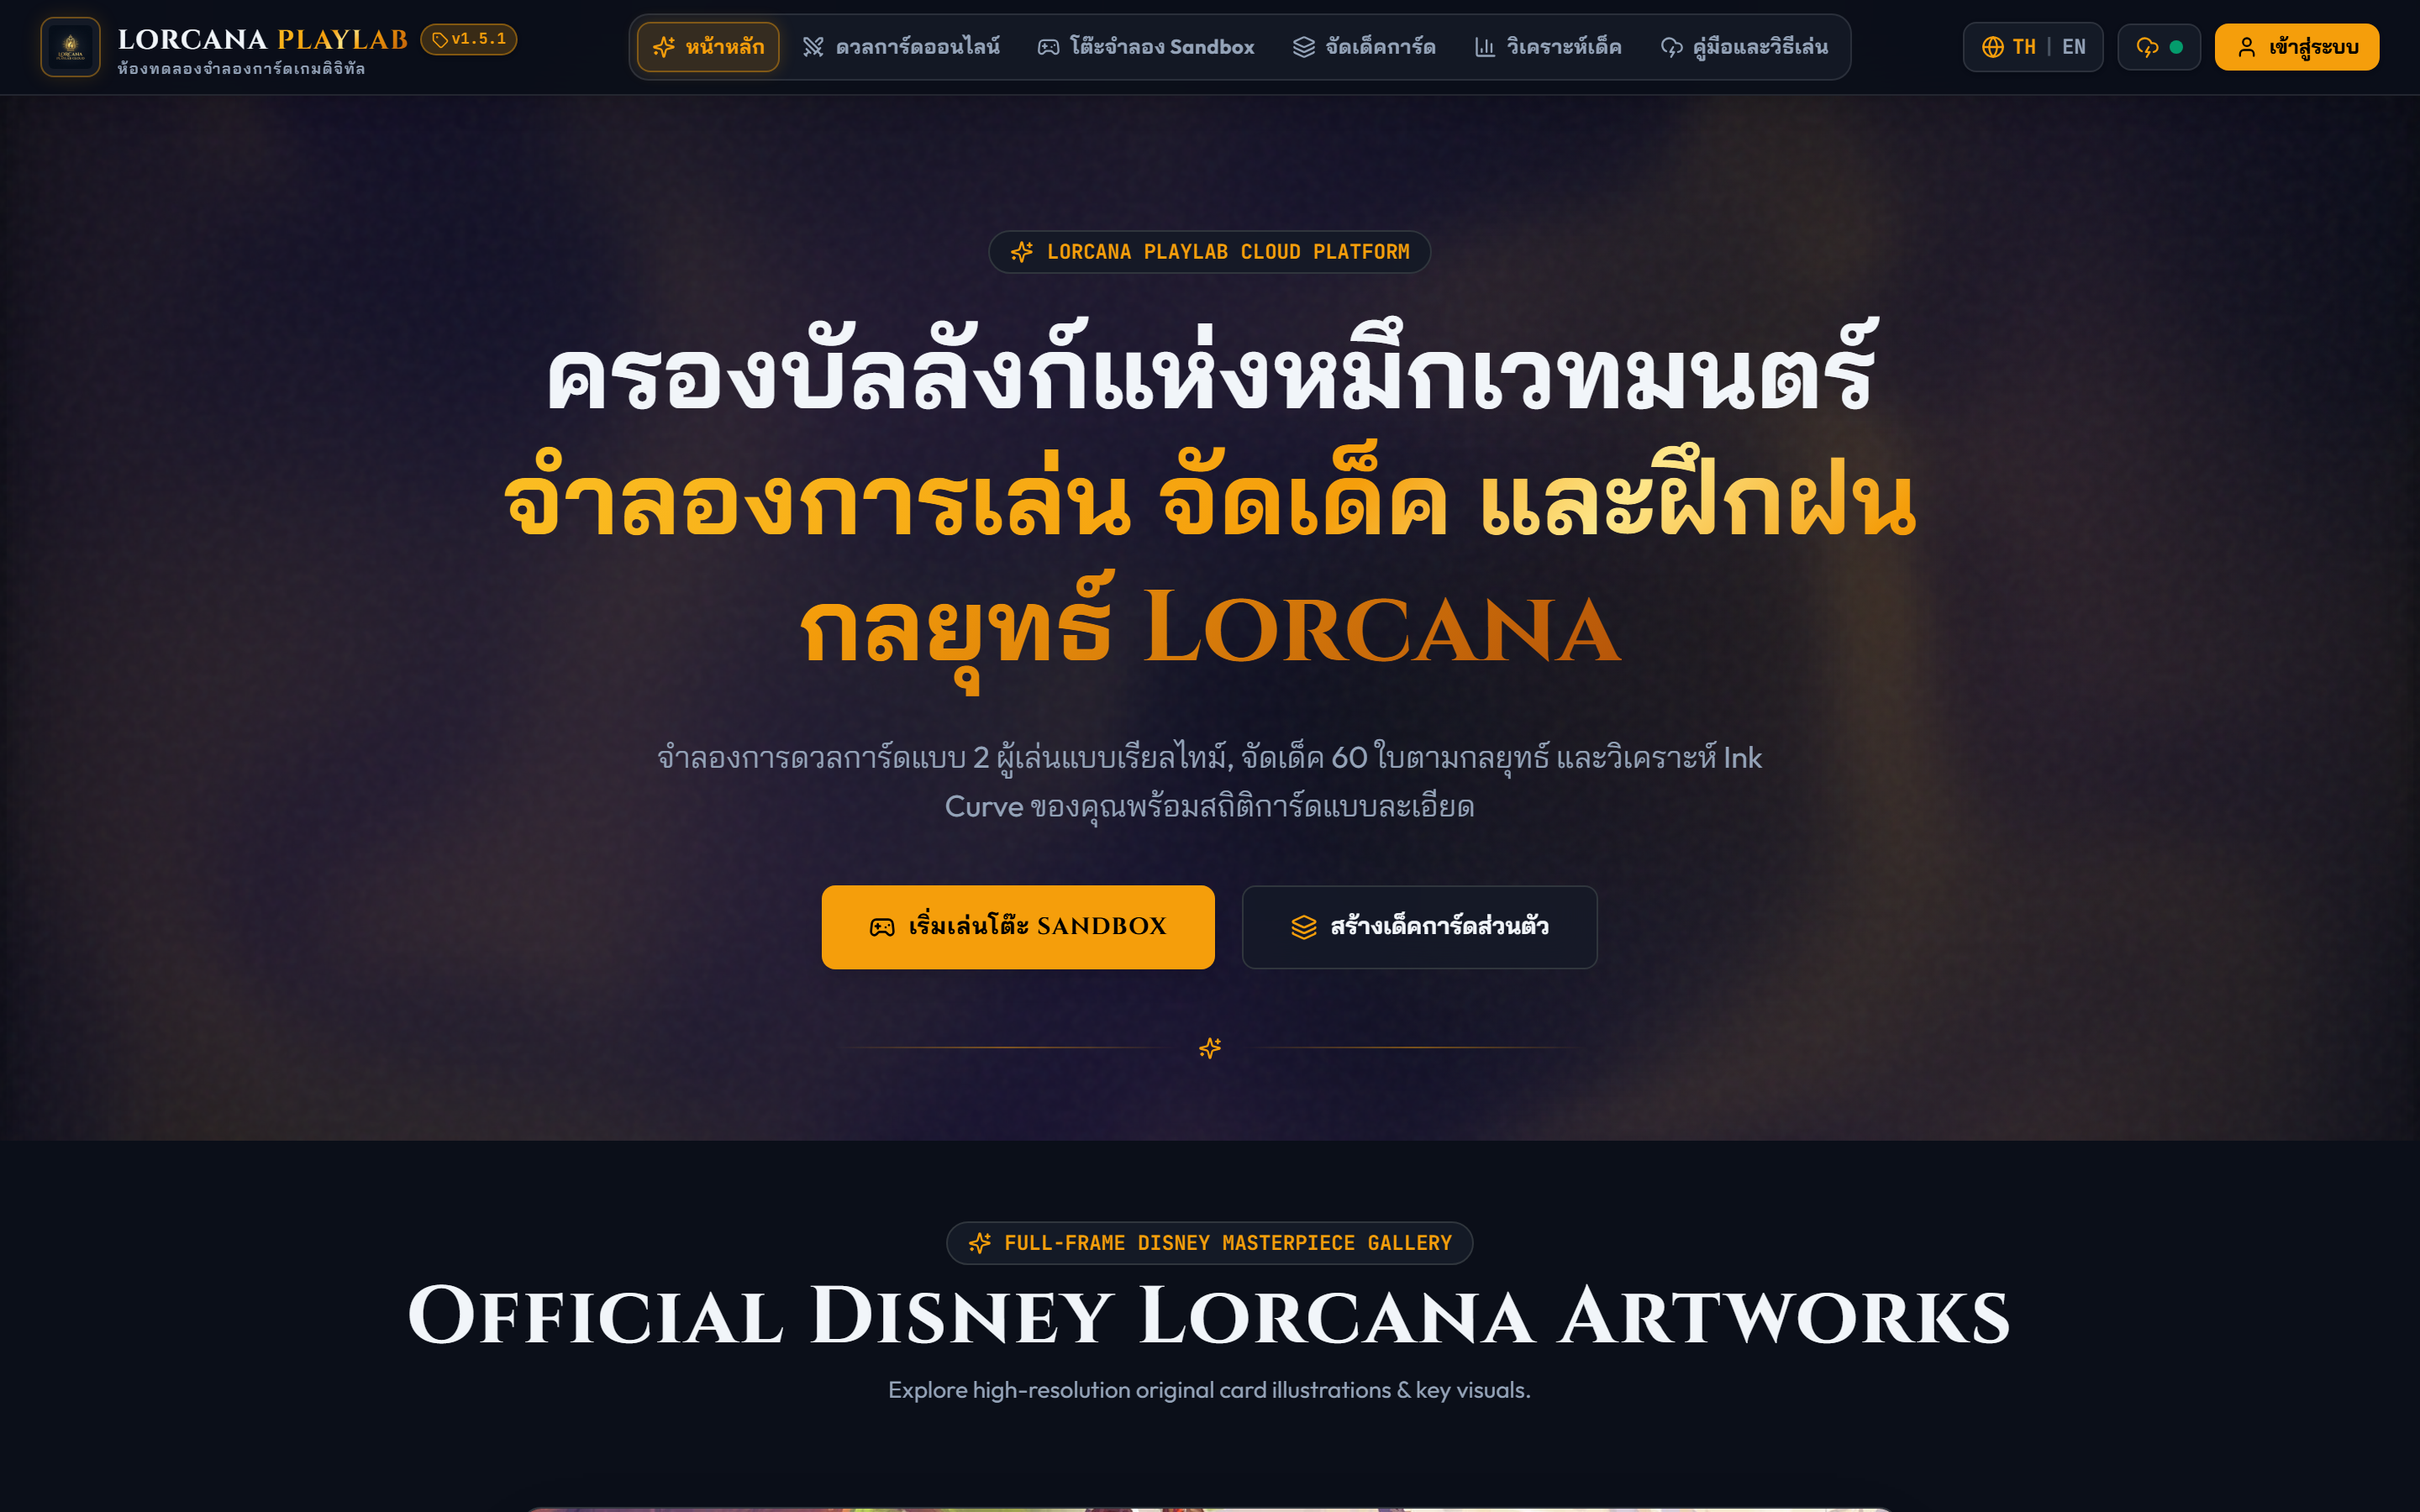
\includegraphics[width=\textwidth]{images/useindoc/01_game_hub_before_login.png}
    \caption{หน้าแรก (Game Hub)}
\end{subfigure}
\hfill
\begin{subfigure}[b]{0.48\textwidth}
    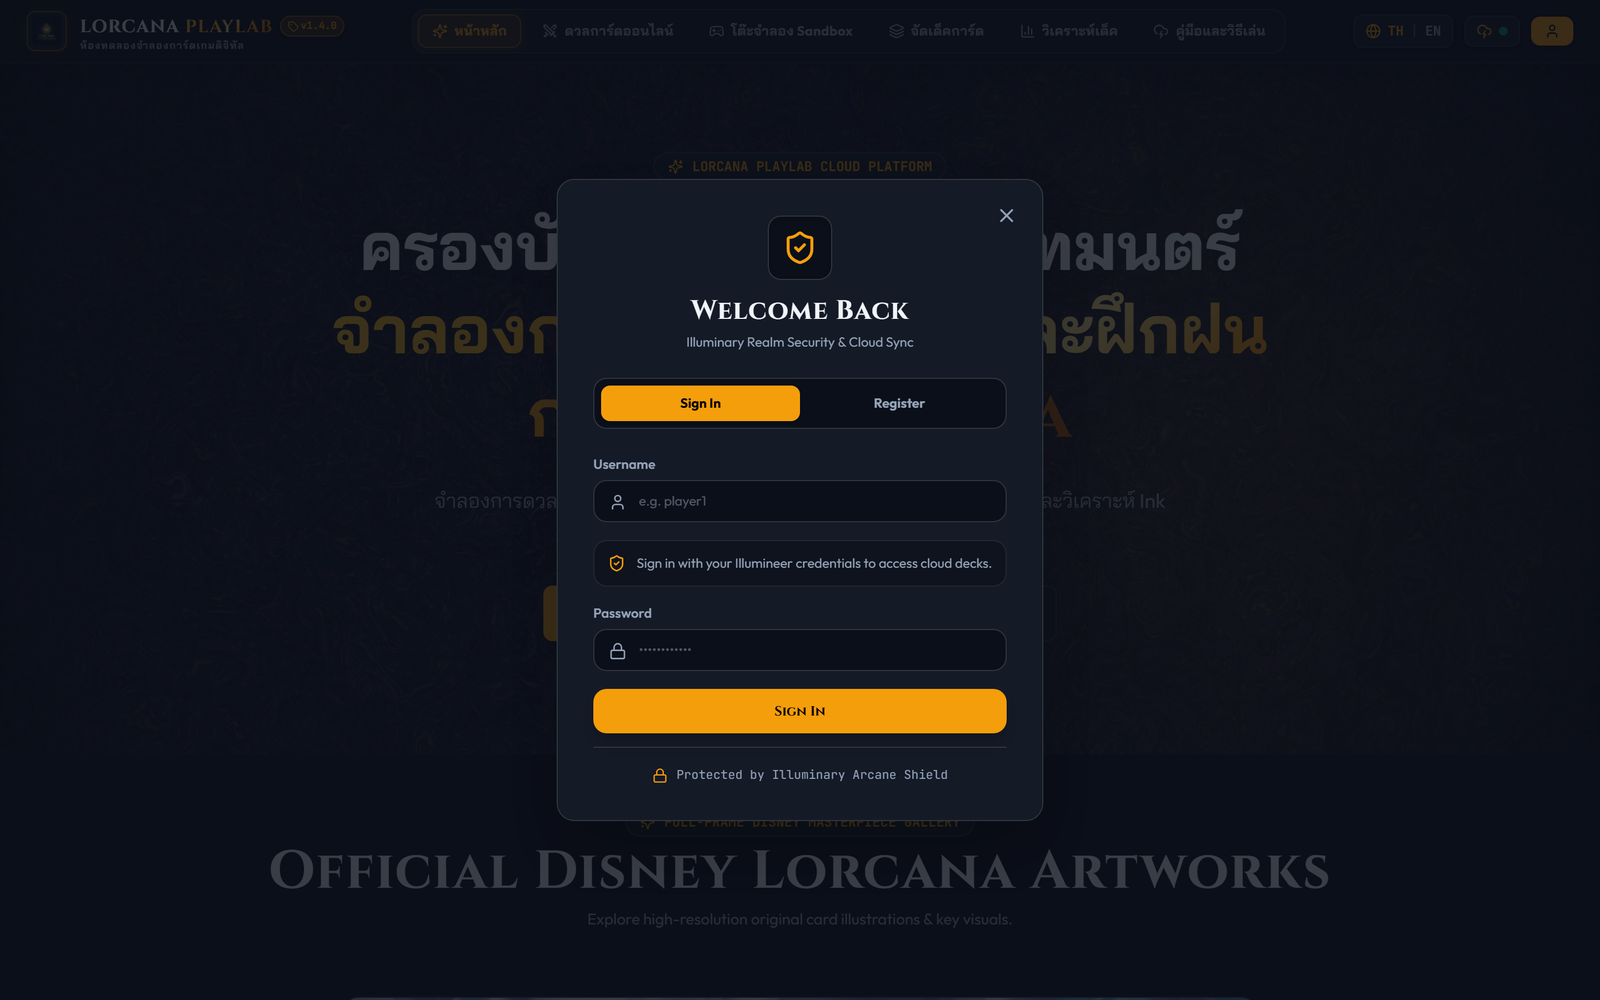
\includegraphics[width=\textwidth]{images/useindoc/02_login_modal.png}
    \caption{หน้าต่างเข้าสู่ระบบ}
\end{subfigure}
\\[0.3cm]
\begin{subfigure}[b]{0.48\textwidth}
    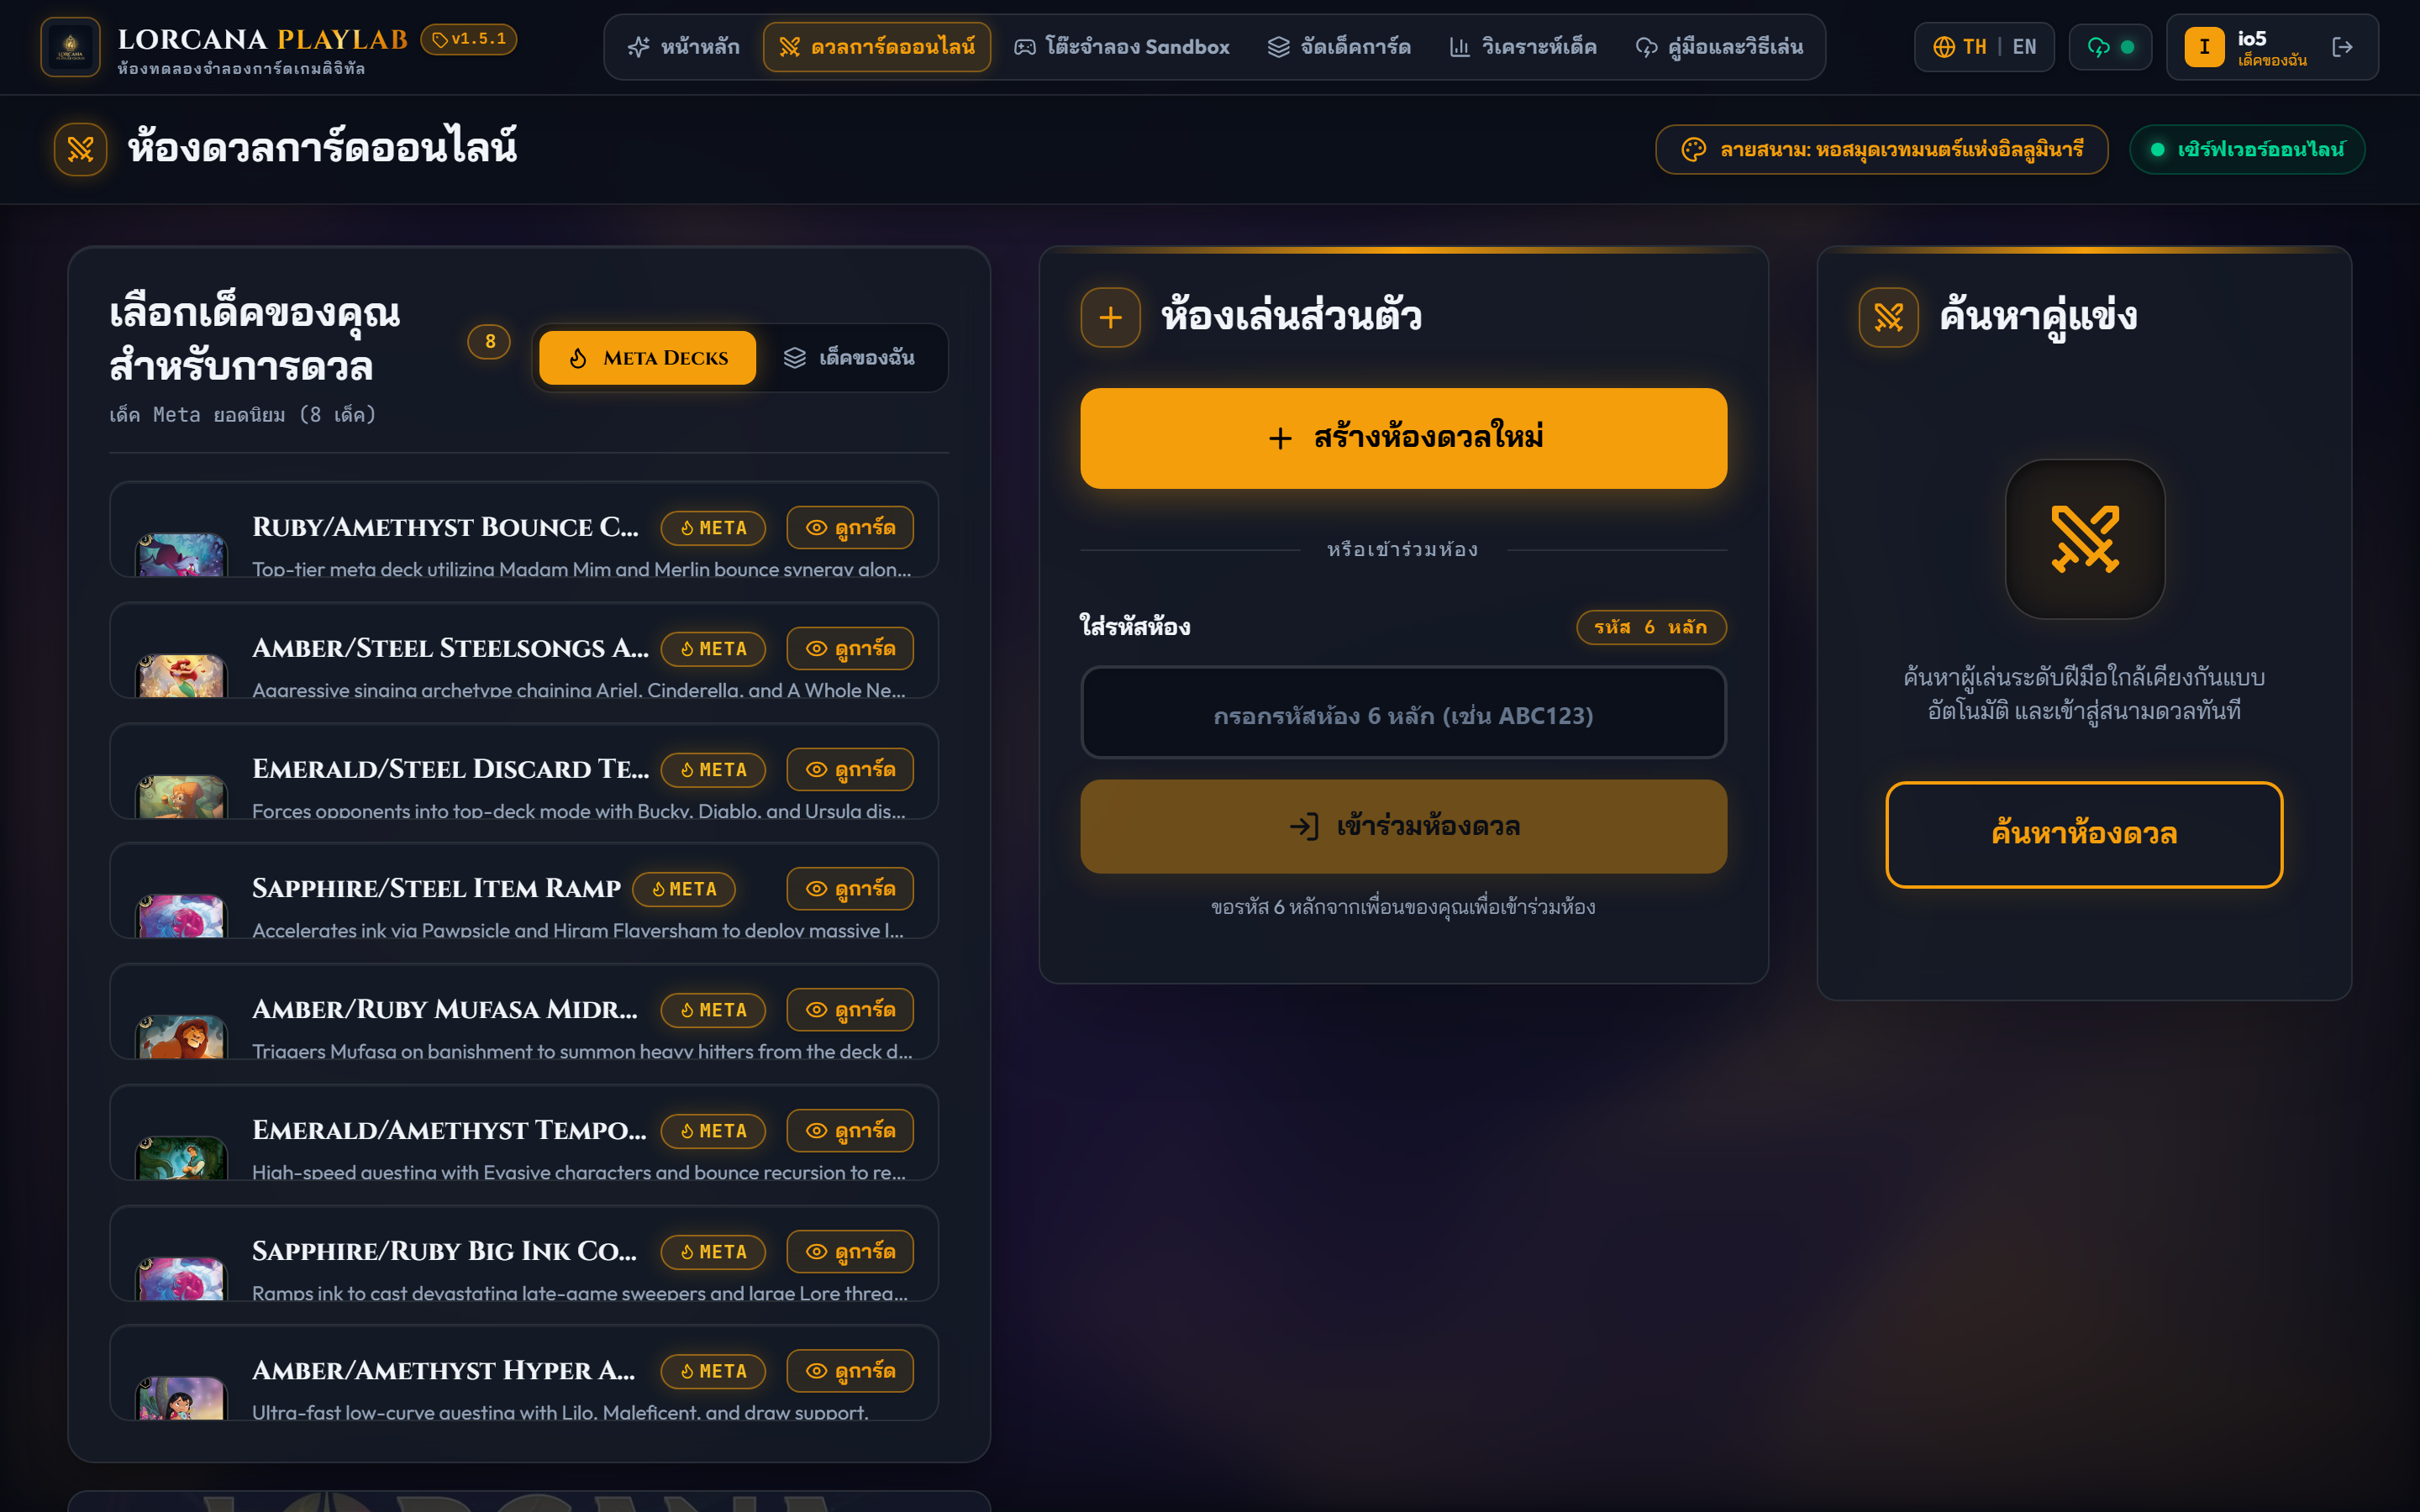
\includegraphics[width=\textwidth]{images/useindoc/05_match_lobby.png}
    \caption{ล็อบบี้สร้างและเข้าห้อง}
\end{subfigure}
\hfill
\begin{subfigure}[b]{0.48\textwidth}
    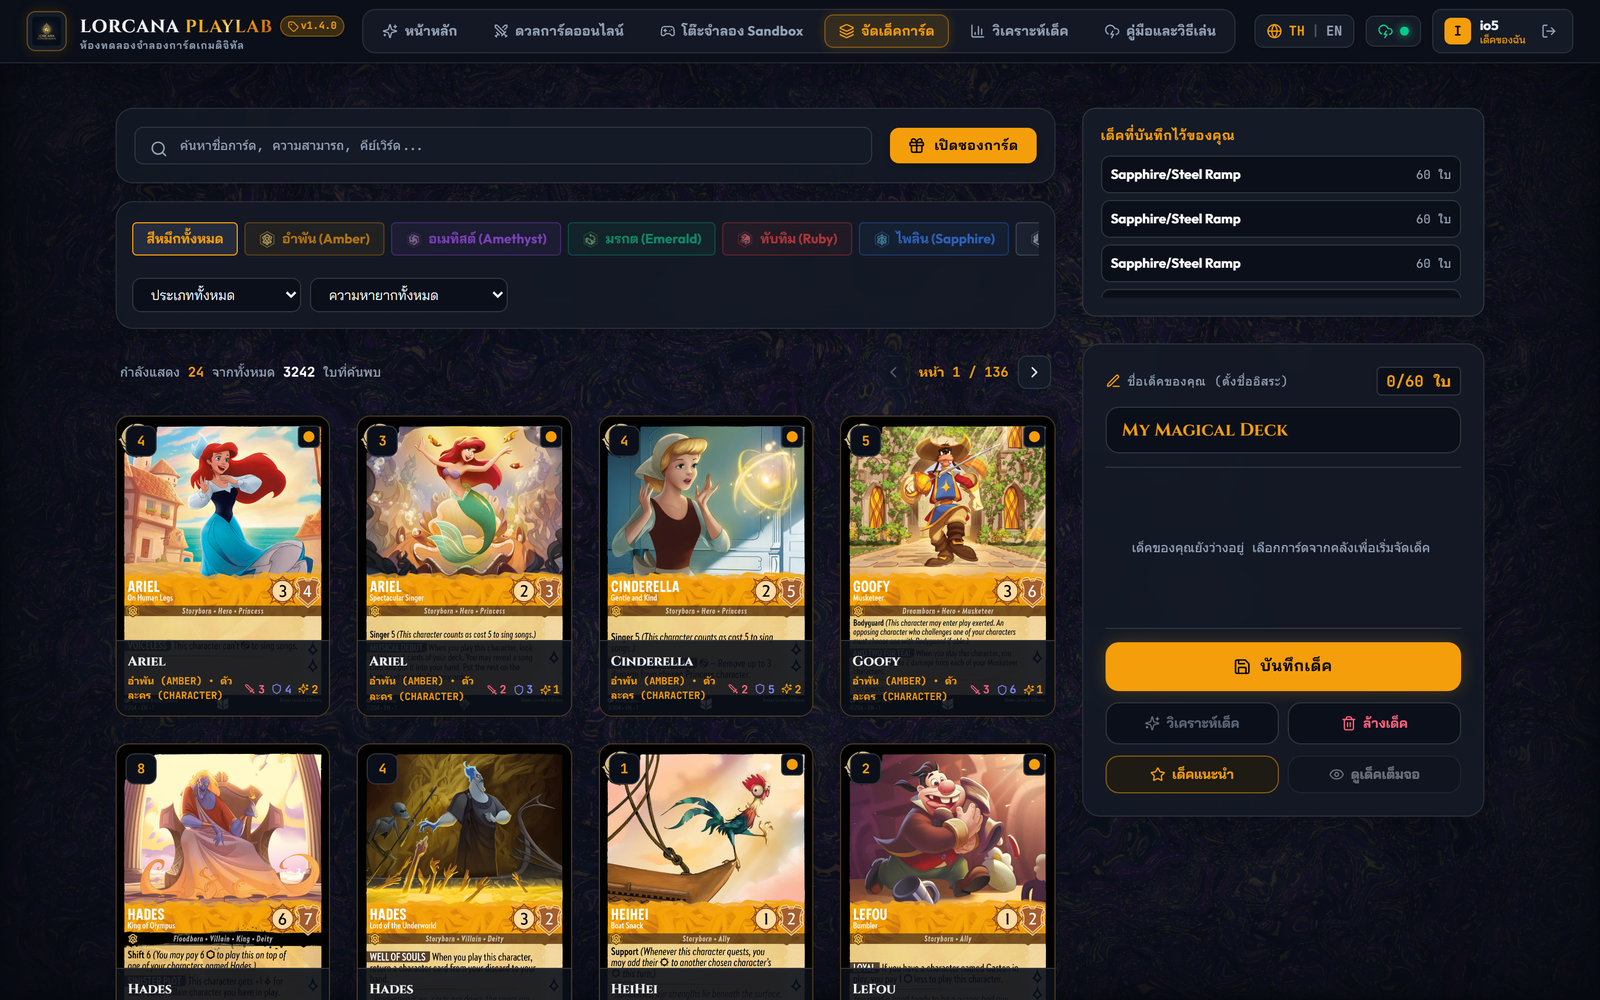
\includegraphics[width=\textwidth]{images/useindoc/04_deck_builder.png}
    \caption{หน้าจัดเด็ค (Deck Builder)}
\end{subfigure}
\\[0.3cm]
\begin{subfigure}[b]{0.48\textwidth}
    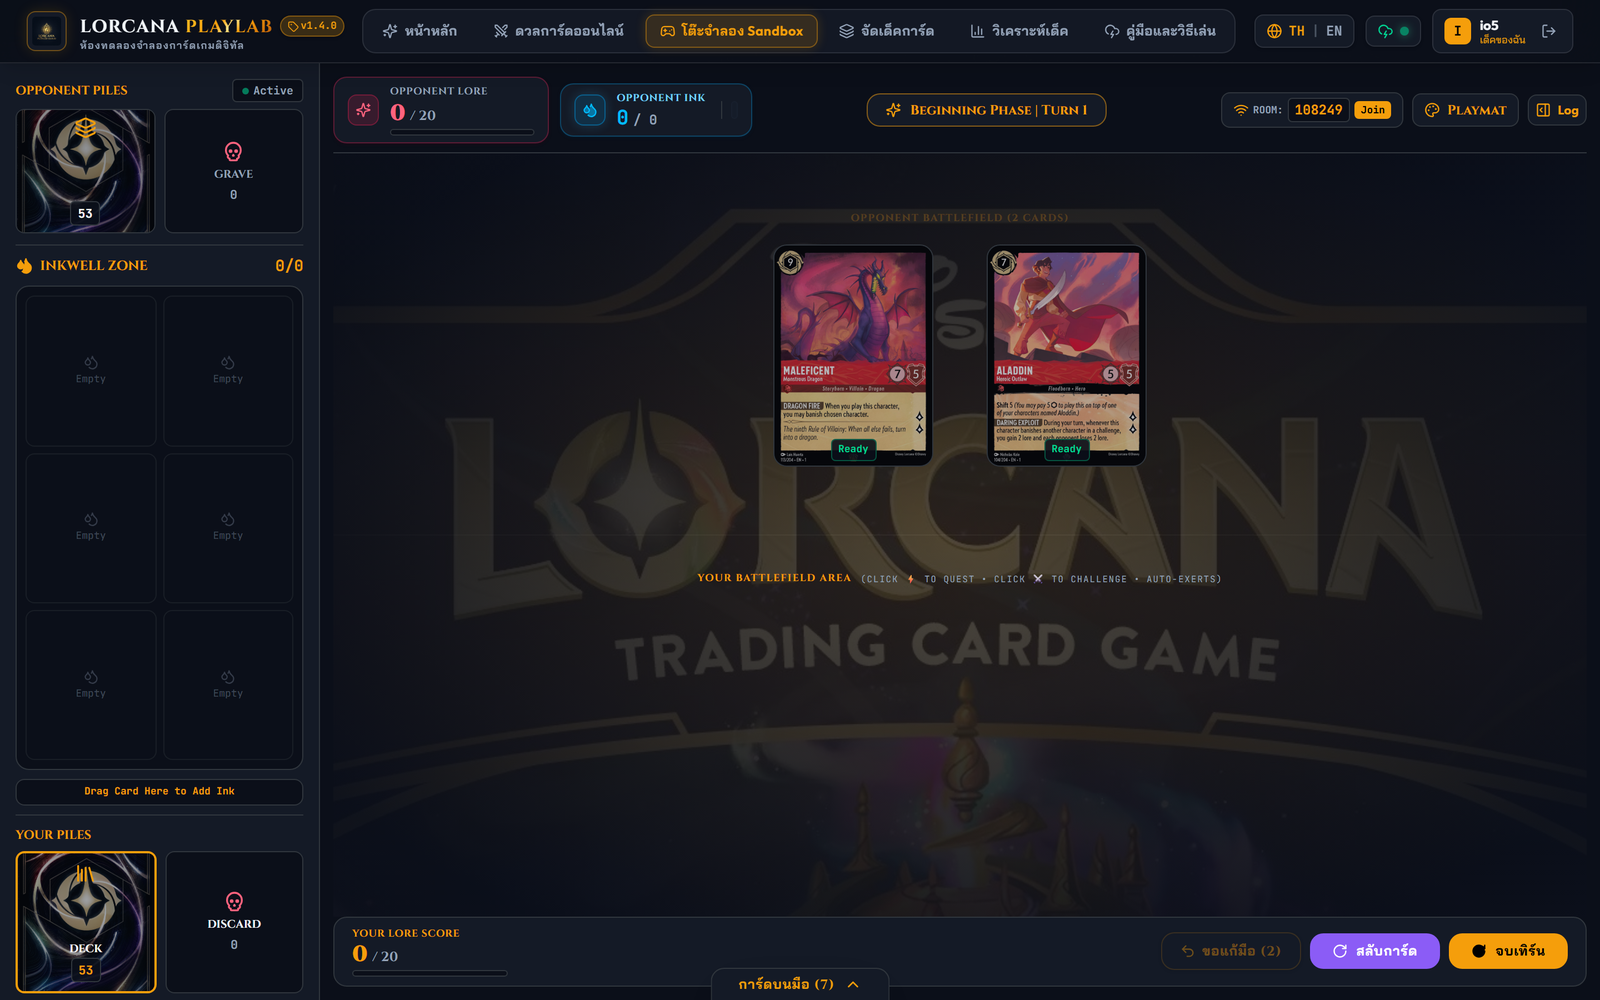
\includegraphics[width=\textwidth]{images/useindoc/07_realtime_room_play.png}
    \caption{กระดานเล่น (Playmat)}
\end{subfigure}
\hfill
\begin{subfigure}[b]{0.48\textwidth}
    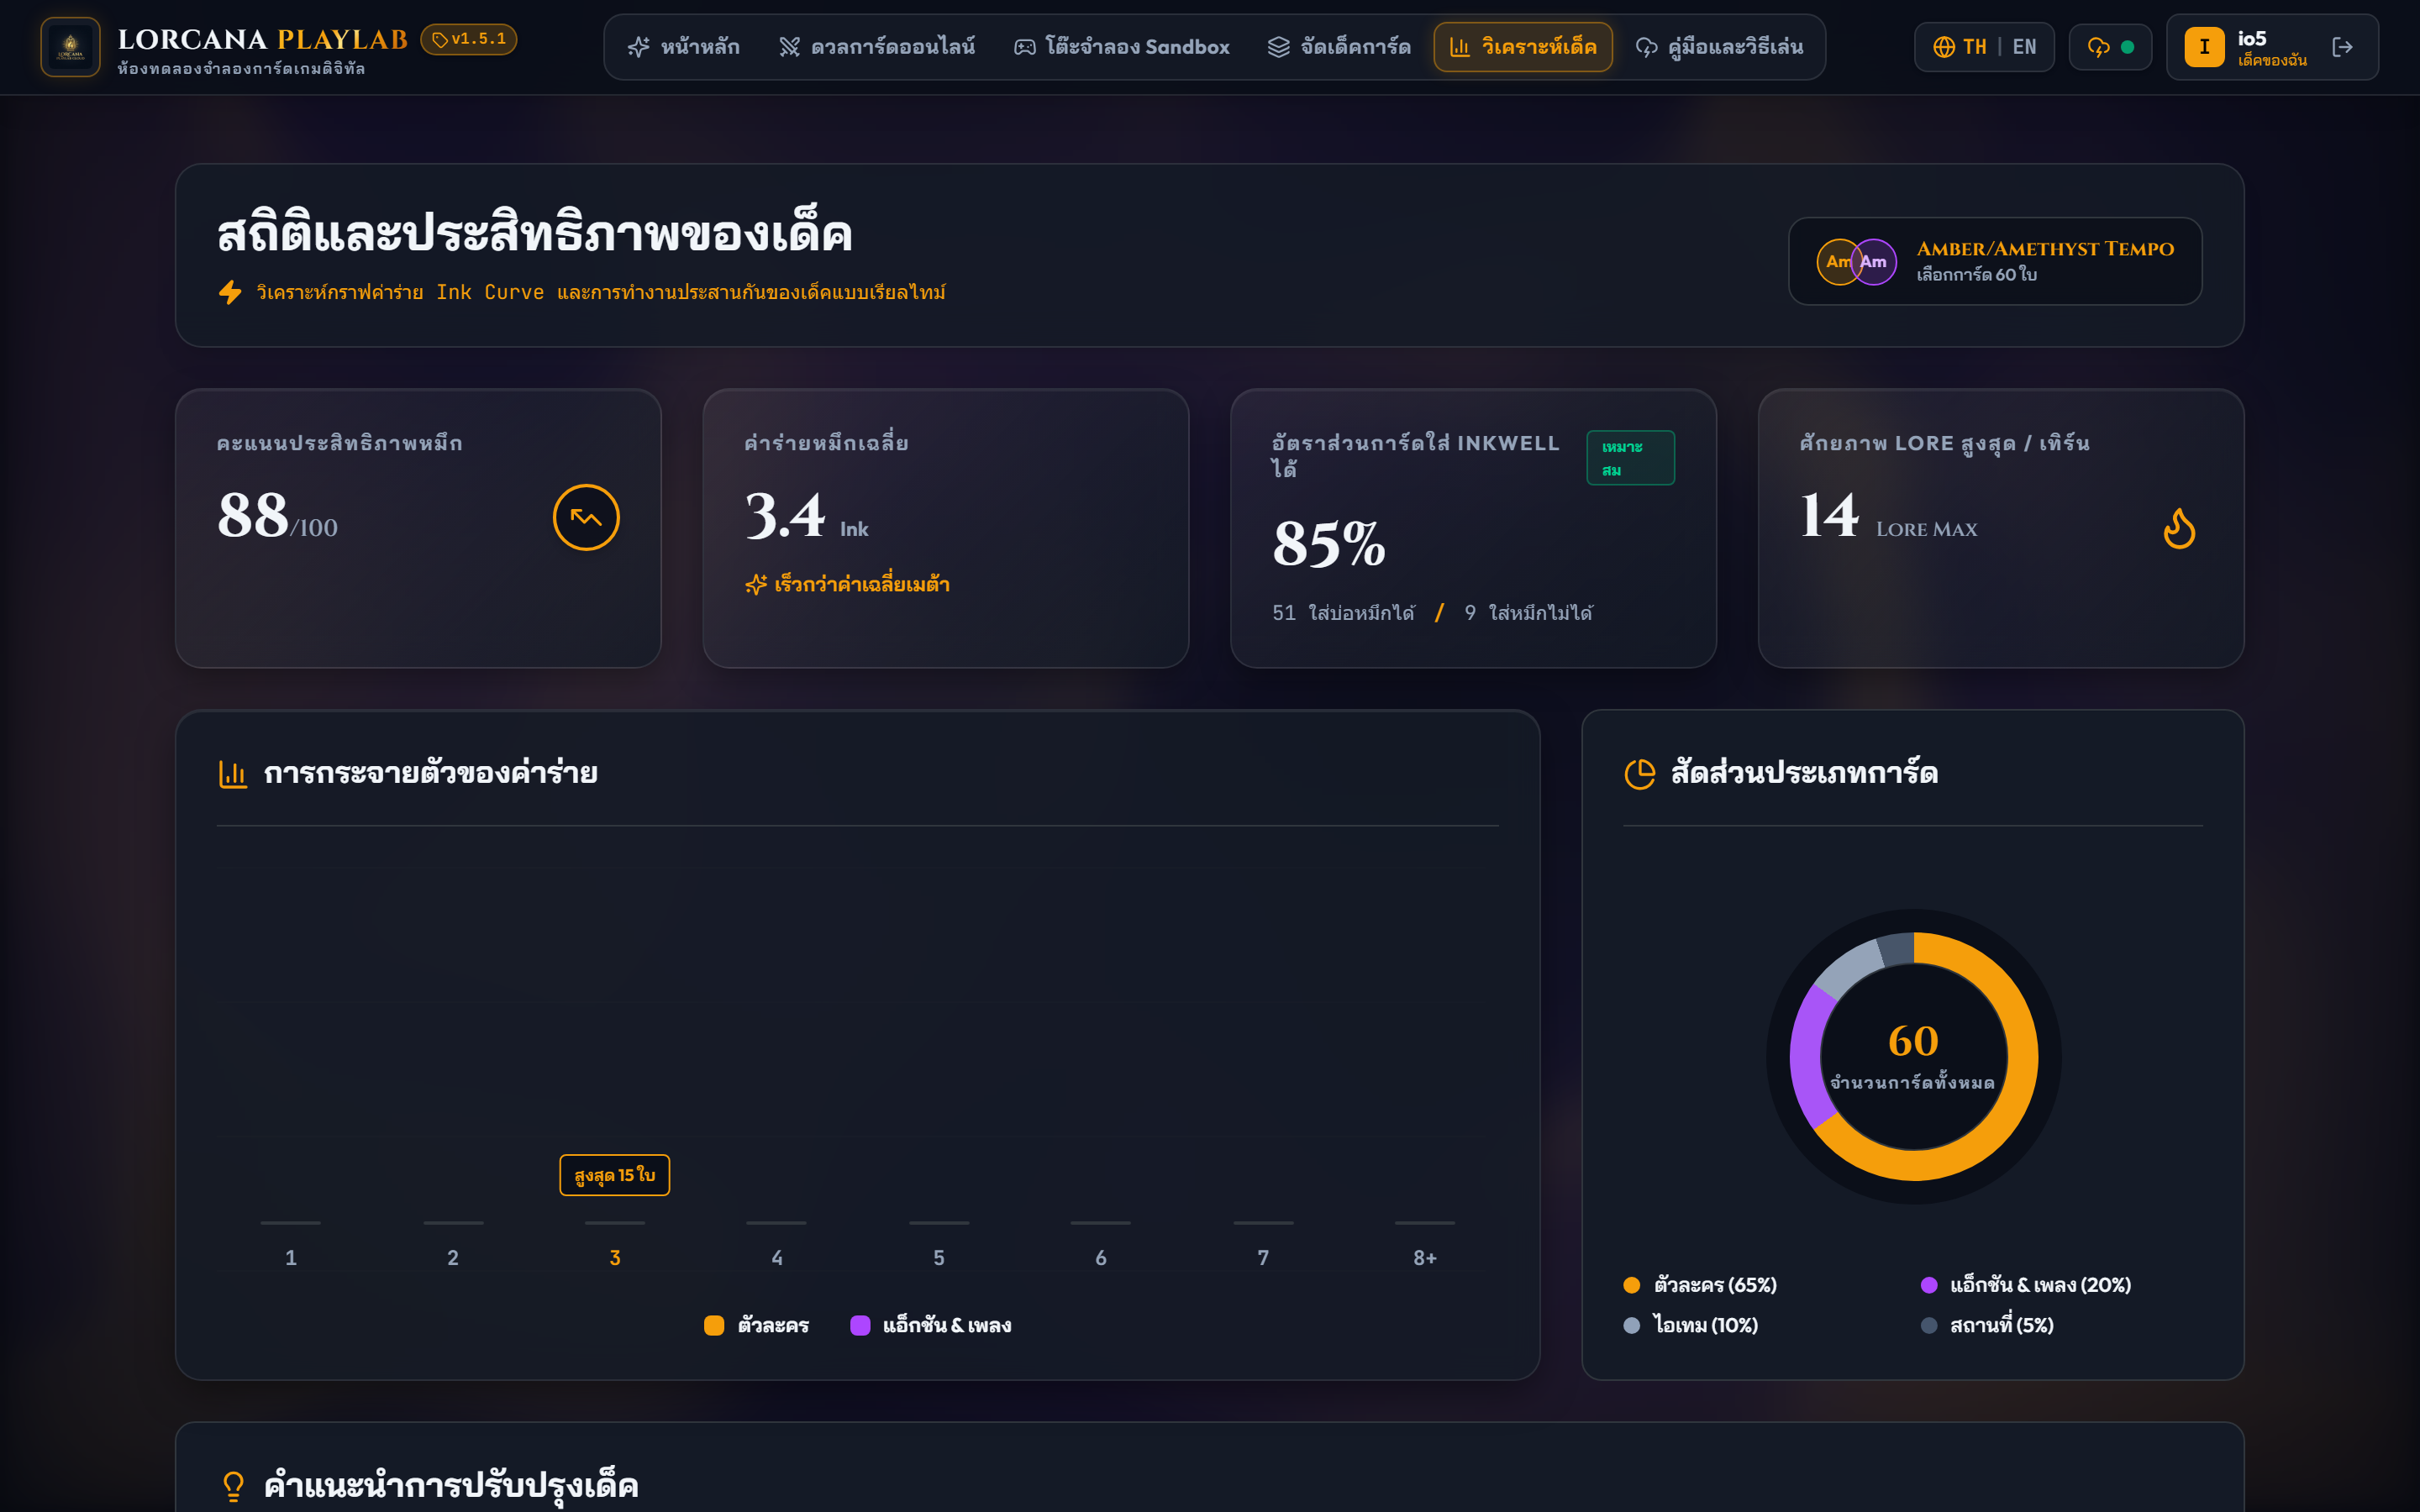
\includegraphics[width=\textwidth]{images/useindoc/09_deck_analytics.png}
    \caption{หน้า Analytics ของเด็ค}
\end{subfigure}
\caption{ภาพหน้าจอของระบบ Disney Lorcana PlayLab Cloud}
\label{fig:ui_showcase}
\end{figure}

องค์ประกอบของกระดานเล่น ได้แก่ พื้นที่สนาม (Play Area) ที่ลากวางการ์ดได้, Inkwell, ตัวนับ Lore 0 ถึง 20, การหมุนการ์ด Ready/Exerted, แถบลำดับเทิร์น (\texttt{TurnPhaseBar}) ที่แสดง \texttt{TURN n}, \texttt{YOUR TURN} และลำดับ Ready, Set, Draw, Main, End (ปุ่มจบเทิร์นอยู่ที่ \texttt{PlayerControlsBar}), หน้าต่าง Dice Duel (\texttt{DiceDuelModal}), หน้าต่าง Mulligan (\texttt{MulliganModal}) และปุ่ม Quest ทุกปุ่มมีป้ายเหตุผลเมื่อทำไม่ได้ เหตุผลมาจากตัวขับเคลื่อนกฎ ไม่ได้เขียนซ้ำใน UI และเล่นครบ 1 เทิร์นได้ด้วยคีย์บอร์ด

ไฟล์ \texttt{LorcanaBoard.tsx} มี 1,617 บรรทัด ณ วันที่ 5 ตุลาคม 2569 \todo{เป้าหมายของ T15 คือต่ำกว่า 1,500 บรรทัด ยังไม่ผ่าน ต้องแยก component เพิ่มก่อนใส่ตัวเลขสุดท้าย}

\section{การทดสอบอัตโนมัติ}

\begin{itemize}
    \item \textbf{Unit และ integration (Vitest 4):} ผ่าน 128 จาก 128 รายการ ใน 20 ไฟล์ (รันเมื่อ 5 ตุลาคม 2569) ครอบคลุมตัวขับเคลื่อนกฎ (TC-ENG), คีย์เวิร์ด (TC-KEY), Ability (TC-AB), Shift/Location/Song/Item (TC-T12), UX (TC-UX), Cache (TC-CACHE) และ Analytics
    \item \textbf{End-to-end (Playwright):} ชุดทดสอบ \texttt{e2e/01} ถึง \texttt{e2e/07} ทำงานกับระบบที่ deploy แล้วเมื่อกำหนด \texttt{E2E\_BASE\_URL} \todo{ใส่จำนวนที่ผ่านทั้งหมดจากการรันรอบสุดท้ายบน stack ที่ deploy ใหม่เมื่อ 5 ตุลาคม 2569}
    \item \textbf{เกมสองผู้เล่น 4 เทิร์น (TC-E2E-25):} เปิด browser สองตัว ทอย Dice Duel เลือก Keep Hand เทิร์น 1 และ 2 ใส่หมึกและลงตัวละคร เทิร์น 3 Quest เทิร์น 4 Challenge ตัวละครที่ Exerted และตรวจว่าหน้าจออีกฝ่ายเห็นการ์ดตรงกัน (\texttt{e2e/07-four-turn-game.spec.ts}) ใช้ 4 เทิร์นเพราะ Challenge เกิดได้เร็วสุดที่เทิร์น 4 (หัวข้อ \ref{sec:challenge}) ชุดทดสอบนี้ไม่ได้ตรวจคีย์เวิร์ดและ Ability เป็นรายใบ เพราะมือเริ่มต้นเป็นการ์ดสุ่ม \textbf{ผล:} ผ่าน 3 จาก 3 รอบติดกันบนระบบที่ deploy เมื่อ 5 ตุลาคม 2569 ใช้เวลา 51.5 ถึง 54.9 วินาทีต่อรอบ (หลักฐาน: \texttt{e2e\_four\_turn\_2026-10-05.txt})
\end{itemize}

ระหว่างสร้างชุดทดสอบ TC-E2E-25 พบข้อบกพร่องในแอป 2 จุด ซึ่งแก้และ deploy ในวันเดียวกัน
\begin{enumerate}
    \item \texttt{TurnPhaseBar} (งาน T13) ผ่าน unit test แต่ไม่เคยถูกแสดงบนกระดานจริง เพราะ \texttt{LorcanaBoard.tsx} import ไว้โดยไม่ได้ใช้ unit test ทดสอบ component เดี่ยวจึงไม่จับข้อนี้ ปัจจุบันแสดงเหนือสนามฝั่งคู่ต่อสู้
    \item ป้ายรายละเอียดการ์ด (quick-glance tooltip) ค้างอยู่หลังการ์ดที่ถูกชี้ออกจากมือ (ลงสนามหรือใส่หมึก) และทับปุ่มจบเทิร์น เพราะการ์ดหายไปก่อนเกิด \texttt{mouseleave} แก้โดยล้างค่าเมื่อการ์ดนั้นไม่อยู่ในมือหรือบนสนามแล้ว
\end{enumerate}
ทั้งสองข้อแสดงว่า unit test ของ component เดี่ยวไม่พอสำหรับยืนยันว่าฟีเจอร์ใช้งานได้ในหน้าจริง ต้องมี end-to-end ที่เล่นผ่านหน้าจอด้วย

\section{การทดลองบน AWS}

การทดลองที่ 1 ถึง 10 ดำเนินการวันที่ 27 และ 29 กันยายน 2569 บน AWS Academy Learner Lab (us-east-1) ไฟล์หลักฐานดิบอยู่ใน \texttt{docs/01\_Reports/stage3\_evidence/}

\subsection{การทดลองที่ 1: เล่นข้ามเครื่อง}

\textbf{คำถาม:} เมื่อมี EC2 2 เครื่อง ผู้เล่นที่ ALB ส่งไปคนละเครื่องเล่นด้วยกันได้หรือไม่

\textbf{วิธี:} Playwright เปิด browser 2 context ผ่าน ALB ผู้เล่น 1 สร้างห้อง ผู้เล่น 2 เข้าด้วยรหัส 6 หลัก ตรวจว่าผู้เล่น 1 เห็นชื่อผู้เล่น 2 ภายใน 10 วินาที

\textbf{ผล:} ผ่าน 5 จาก 5 รอบ ใช้เวลา 9.7 ถึง 14.1 วินาทีต่อรอบ (รวมสมัครสมาชิก เข้าสู่ระบบ และโหลดหน้า) \todo{ไม่มีไฟล์ log ดิบของการทดลองนี้ใน \texttt{stage3\_evidence/} ควรรันซ้ำและเก็บ log}

\subsection{การทดลองที่ 2: ความปลอดภัยบนระบบจริง}

\begin{table}[H]
\centering
\caption{ผลทดสอบความปลอดภัย (OWASP Top 10 [10]: A02, A05, A07)}
\begin{tabularx}{\textwidth}{lX}
\toprule
\textbf{Test Case} & \textbf{ผล} \\
\midrule
TC-AUTH-00a: backend รันโดยไม่มี secret & ก่อนแก้ รันต่อได้ (FAIL) หลังแก้ ออกด้วย exit 1 (PASS) \\
TC-AUTH-00c: รหัส admin ที่เขียนไว้ในโค้ด & ถูกปฏิเสธ (PASS) \\
TC-E2E-16: JWT ที่เซ็นด้วย secret ค่าเริ่มต้น & ได้ 401 ทุกรอบ (10 จาก 10 รอบ) \\
TC-E2E-16: security headers & \texttt{X-Frame-Options: DENY}, \texttt{X-Content-Type-Options: nosniff} \\
Launch template & \texttt{HttpTokens: required} และไม่มี secret ใน user data \\
\bottomrule
\end{tabularx}
\end{table}

\subsection{การทดลองที่ 3: Failover เมื่อ backend ล่ม}

สคริปต์ \texttt{test\_asg\_recovery.ps1} สั่ง \texttt{systemctl stop lorcana-backend} บนเครื่องหนึ่งผ่าน SSM Run Command แล้วจับเวลาจนเครื่องใหม่ healthy และ alarm กลับเป็น OK

\begin{table}[H]
\centering
\caption{ผลการทดลอง Failover (หลักฐาน: \texttt{failover\_app\_*.txt})}
\begin{tabularx}{\textwidth}{lXX}
\toprule
\textbf{เหตุการณ์} & \textbf{รอบ 1 (08:32:50)} & \textbf{รอบ 2 (11:22:57)} \\
\midrule
ASG สั่งเปลี่ยนเครื่อง & T+146 วินาที & T+90 วินาที \\
เครื่องใหม่ healthy & T+231 วินาที & T+166 วินาที \\
Alarm กลับเป็น OK & T+428 วินาที & T+354 วินาที \\
\bottomrule
\end{tabularx}
\end{table}

ALB หยุดส่งทราฟฟิกไปเครื่องที่ล่มภายในราว 30 วินาที (health check 15 วินาที สองครั้ง) ช่วงนั้นคำขออาจได้ 502 เวลากู้คืน 2.8 ถึง 3.9 นาที ส่วนใหญ่เป็นเวลาบูตเครื่องใหม่

\subsection{การทดลองที่ 4: Auto Scaling}

ใช้ \texttt{POST /api/auth/login} (bcrypt cost 10 ใช้ CPU จริง) จาก 40 worker ต่อเนื่อง

\begin{table}[H]
\centering
\caption{ผลการทดลอง Auto Scaling (หลักฐาน: \texttt{stress\_scaling\_*.txt})}
\begin{tabularx}{\textwidth}{lXX}
\toprule
& \textbf{รอบ 1 (process เดียว)} & \textbf{รอบ 2 (cluster 2 worker)} \\
\midrule
CPU เฉลี่ย & 48.7--49.9\% (ค้าง) & 99.8--99.97\% \\
Scale-out & ไม่เกิด & 2 เป็น 4 เครื่อง \\
Login สำเร็จ/ล้มเหลว & ไม่ได้บันทึก & 9,653/0 \\
\bottomrule
\end{tabularx}
\end{table}

\subsection{การทดลองที่ 5: Infrastructure as Code}

\texttt{deploy\_ec2\_vpc\_asg.ps1} สร้าง VPC, subnet 2 AZ, IGW, Security Group, ALB, Target Group, Launch Template, ASG, scaling policy และ alarm สำเร็จ รันซ้ำขณะ stack ยังอยู่จะหยุดด้วย exit 1 ส่วน \texttt{lab.ps1 destroy} ลบทรัพยากรทั้งหมดเหลือแค่ default VPC

เมื่อสร้าง stack ใหม่วันที่ 5 ตุลาคม 2569 พบบั๊กในสคริปต์ \texttt{ensure\_pipeline.ps1}: ตาราง \texttt{LorcanaMatchHistory} และ \texttt{LorcanaPlayerStats} ถูกสร้างด้วยชื่อ key เป็นข้อความ \texttt{\$PkName} ตรงตัว เพราะ PowerShell 7 ไม่แทนค่าตัวแปรในอาร์กิวเมนต์ที่ไม่มีเครื่องหมายคำพูด Lambda ที่ใช้ key \texttt{userId} จึงเขียนตารางไม่ได้ แก้โดยใส่เครื่องหมายคำพูดครอบอาร์กิวเมนต์ แล้วสร้างตารางใหม่ ตรวจ key ได้ \texttt{userId} (และ \texttt{finishedAt\#matchId}) ถูกต้อง

\subsection{การทดลองที่ 6: Content Caching}

\begin{table}[H]
\centering
\caption{ผล Content Caching (หลักฐาน: \texttt{caching\_2026-09-29*.json})}
\begin{tabularx}{\textwidth}{lX}
\toprule
\textbf{ตัวชี้วัด} & \textbf{ค่า} \\
\midrule
ขนาดไฟล์ข้อมูลการ์ดก่อนบีบอัด & 2,351,188 ไบต์ (2.35 MB) \\
ขนาดหลัง gzip & 436,557 ไบต์ (426 KB) ลดลง 81.43\% \\
เวลาโหลดครั้งแรก & 602 มิลลิวินาที \\
เวลาโหลดครั้งที่สอง (cache hit) & 86 มิลลิวินาที \\
ข้อมูลรับส่งครั้งที่สอง & 0 ไบต์ (ใช้แคชในเบราว์เซอร์) \\
\bottomrule
\end{tabularx}
\end{table}

\subsection{การทดลองที่ 7: Dead Letter Queue}

ข้อความ JSON เสียหายถูกส่งเข้าคิววิเคราะห์เด็ค Lambda ส่งคืน \texttt{batchItemFailures} ข้อความถูกลองซ้ำครบ 3 ครั้ง (\texttt{maxReceiveCount: 3}) แล้วเข้า DLQ ที่ T+102 วินาที จำนวนข้อความค้างในคิวหลัก 0 ข้อความ (หลักฐาน: \texttt{dlq\_20260929\_131824.log})

\subsection{การทดลองที่ 8: SNS Fan-out}

เทสต์ TC-E2E-23 (สมัคร เข้าสู่ระบบ สร้างเด็ค จบเกม แล้วรอจนผลปรากฏในประวัติและสถิติของทั้งสองผู้เล่น) ใช้เวลารวม 4.9 วินาที จึงสรุปได้ว่าการกระจายผลใช้เวลาไม่เกิน 5 วินาทีหลังจบเกม (ยังไม่ได้แยกวัดเฉพาะช่วง SNS ถึง DynamoDB) การป้องกันการเข้าถึง (OWASP A01): ส่งผลโดยไม่มี JWT ได้ 401 ส่งผลของแมตช์ที่ตนไม่ได้เล่นได้ 403 (หลักฐาน: \texttt{decoupling\_match\_events\_20260929.log})

\subsection{การทดลองที่ 9: ElastiCache แบบ Cache-Aside}

\textbf{วิธี:} \texttt{measure\_leaderboard.mjs} เรียก \texttt{GET /api/leaderboard} ผ่าน ALB 8 รอบ แต่ละรอบรอให้ TTL 60 วินาทีหมดก่อน 1 คำขอ (ควรได้ MISS) แล้วยิงต่อเนื่อง 13 คำขอ (ควรได้ HIT) แยกกลุ่มตาม header \texttt{X-Cache} ที่ server ตอบ ค่า \texttt{durationMs} วัดภายใน backend ส่วนค่าฝั่ง client รวมความหน่วงเครือข่ายด้วย

\begin{table}[H]
\centering
\caption{ผลตารางผู้นำ (ค่ามัธยฐานและ p95 หลักฐาน: \nolinkurl{leaderboard_cache_2026-09-29T17-18-08-612Z.json})}
\begin{tabularx}{\textwidth}{Xrrr}
\toprule
\textbf{สถานการณ์} & \textbf{ตัวอย่าง} & \textbf{server (p95)} & \textbf{client (p95)} \\
\midrule
Cache Miss (อ่าน DynamoDB) & 8 & 41 ms (112) & 562.7 ms (814.2) \\
Cache Hit (ภายใน TTL 60 วินาที) & 104 & 1 ms (2) & 247.5 ms (255.9) \\
\bottomrule
\end{tabularx}
\end{table}

เวลาฝั่ง server ลดจาก 41 เหลือ 1 มิลลิวินาที (ลดลง 97.56\%) เวลาที่ผู้ใช้เห็นลดจาก 562.7 เหลือ 247.5 มิลลิวินาที เพราะความหน่วงเครือข่ายราว 247 มิลลิวินาทีแคชลดไม่ได้ กลุ่ม MISS มีเพียง 8 ตัวอย่างเพราะต้องรอ TTL 62 วินาทีต่อ 1 ตัวอย่าง และตารางสถิติมีข้อมูลน้อย ค่า MISS บนตารางใหญ่กว่านี้จะสูงขึ้น เมื่อแคชขัดข้องระบบอ่าน DynamoDB โดยตรงและตอบ HTTP 200 (ทดสอบด้วย unit test TC-LEAD-04 และ TC-CACHE-004)

\textbf{ปัญหาที่พบ:} รอบแรกได้ MISS ตลอด สาเหตุคือ Redis client เชื่อมต่อตอนมีคำขอแรกและตั้ง \texttt{enableOfflineQueue: false} คำขอแรกของทุก process จึงล้มเงียบแล้วไปอ่าน DynamoDB แก้โดยเชื่อมต่อตอน server เริ่ม (\texttt{warmCache()}) และเพิ่ม unit test TC-CACHE-001 ถึง 004 หลังแก้ TC-E2E-24 ได้ MISS แล้ว HIT ตามที่ออกแบบ

\subsection{การทดลองที่ 10: Ability Coverage}

\texttt{measure\_ability\_coverage.ts} วิเคราะห์การ์ด 3,242 ใบ (Set 1 ถึง 13) พบ Ability 3,768 ข้อ (หลักฐาน: \texttt{ability\_coverage.json})

\begin{table}[H]
\centering
\caption{ระดับการรองรับ Ability ของตัวขับเคลื่อนกฎ}
\begin{tabularx}{\textwidth}{lrX}
\toprule
\textbf{ระดับ} & \textbf{จำนวน (\%)} & \textbf{คำอธิบาย} \\
\midrule
Full Support & 609 (16.16\%) & ระบบคำนวณและเลือกเป้าหมายอัตโนมัติ \\
Partial Support & 203 (5.39\%) & ตรวจจังหวะ trigger ได้ ต้องระบุเพิ่มเติม \\
Manual Resolve & 2,956 (78.45\%) & แสดงป้ายให้ผู้เล่นจัดการเอง \\
\bottomrule
\end{tabularx}
\end{table}

\subsection{ภาพหลักฐานจาก AWS Console}

ภาพในหัวข้อนี้แคปจาก AWS Console ภูมิภาค us-east-1 เมื่อวันที่ 12 ตุลาคม 2569 หลังสร้าง stack ใหม่และ publish โค้ดล่าสุด ภาพอยู่ใน \texttt{docs/01\_Reports/images/useindoc/} ไฟล์ขึ้นต้นด้วย \texttt{aws\_2026-10-12\_}

\begin{figure}[H]
\centering
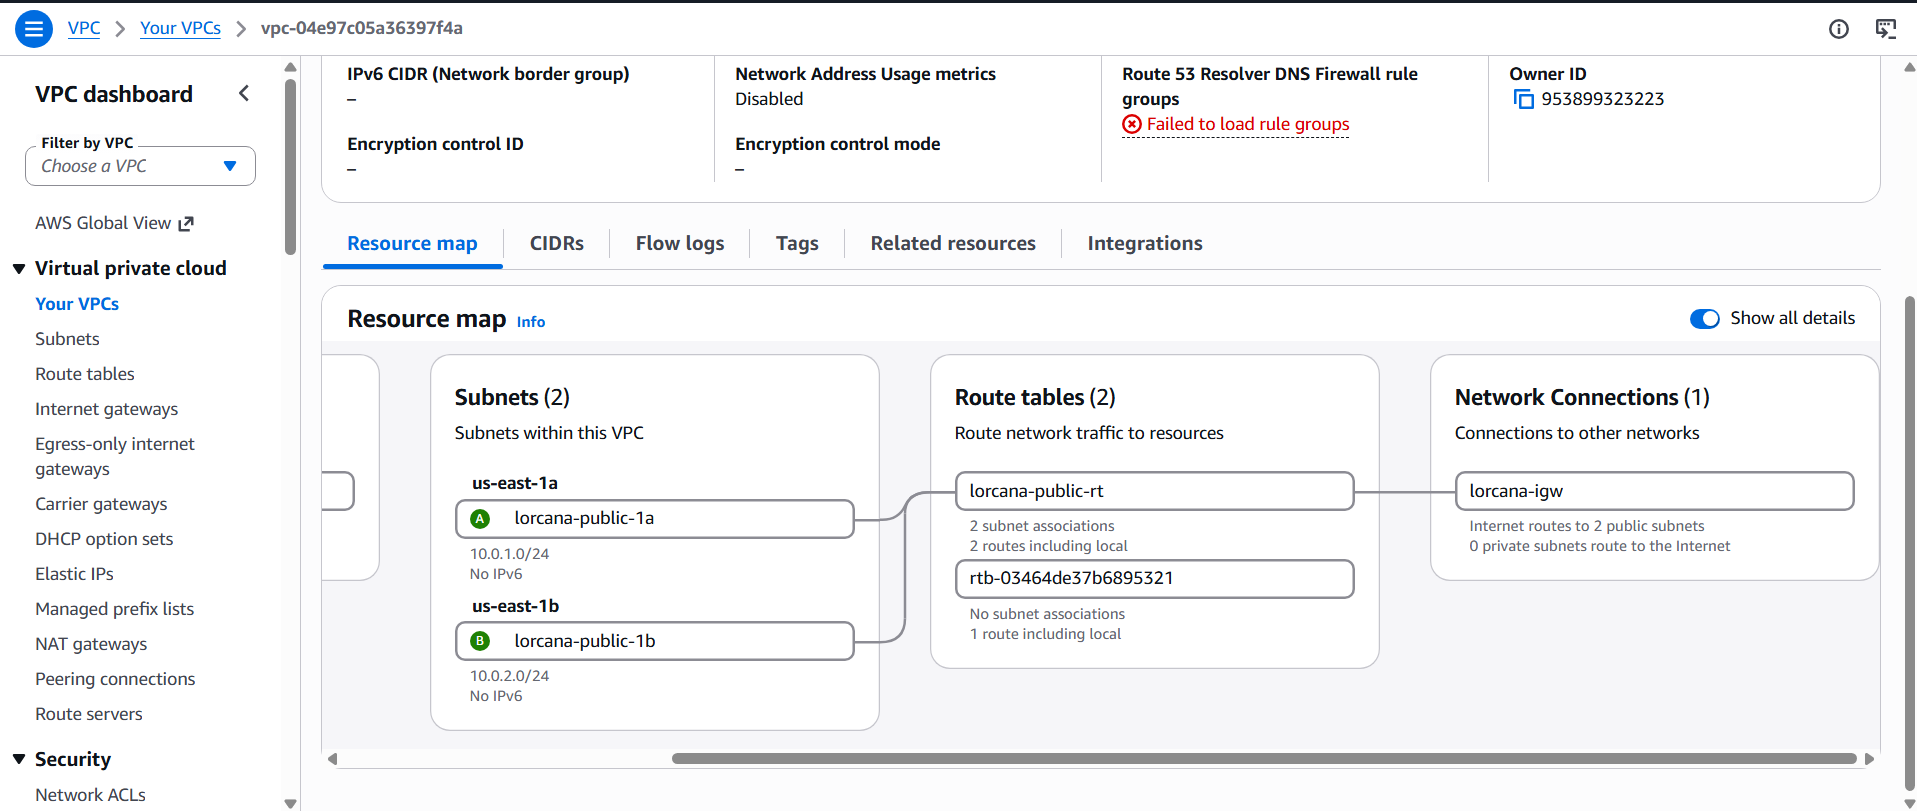
\includegraphics[width=\textwidth]{images/useindoc/aws_2026-10-12_vpc_resource_map.png}
\caption{Resource map ของ VPC \texttt{lorcana-lean-vpc} (10.0.0.0/16): subnet สาธารณะ \texttt{lorcana-public-1a} และ \texttt{lorcana-public-1b} ใน 2 Availability Zone, route table \texttt{lorcana-public-rt} ผูกกับทั้งสอง subnet และเชื่อม \texttt{lorcana-igw} ไม่มี private subnet และไม่มี NAT Gateway}
\label{fig:aws_vpc_map}
\end{figure}

\begin{figure}[H]
\centering
\begin{subfigure}[b]{0.48\textwidth}
    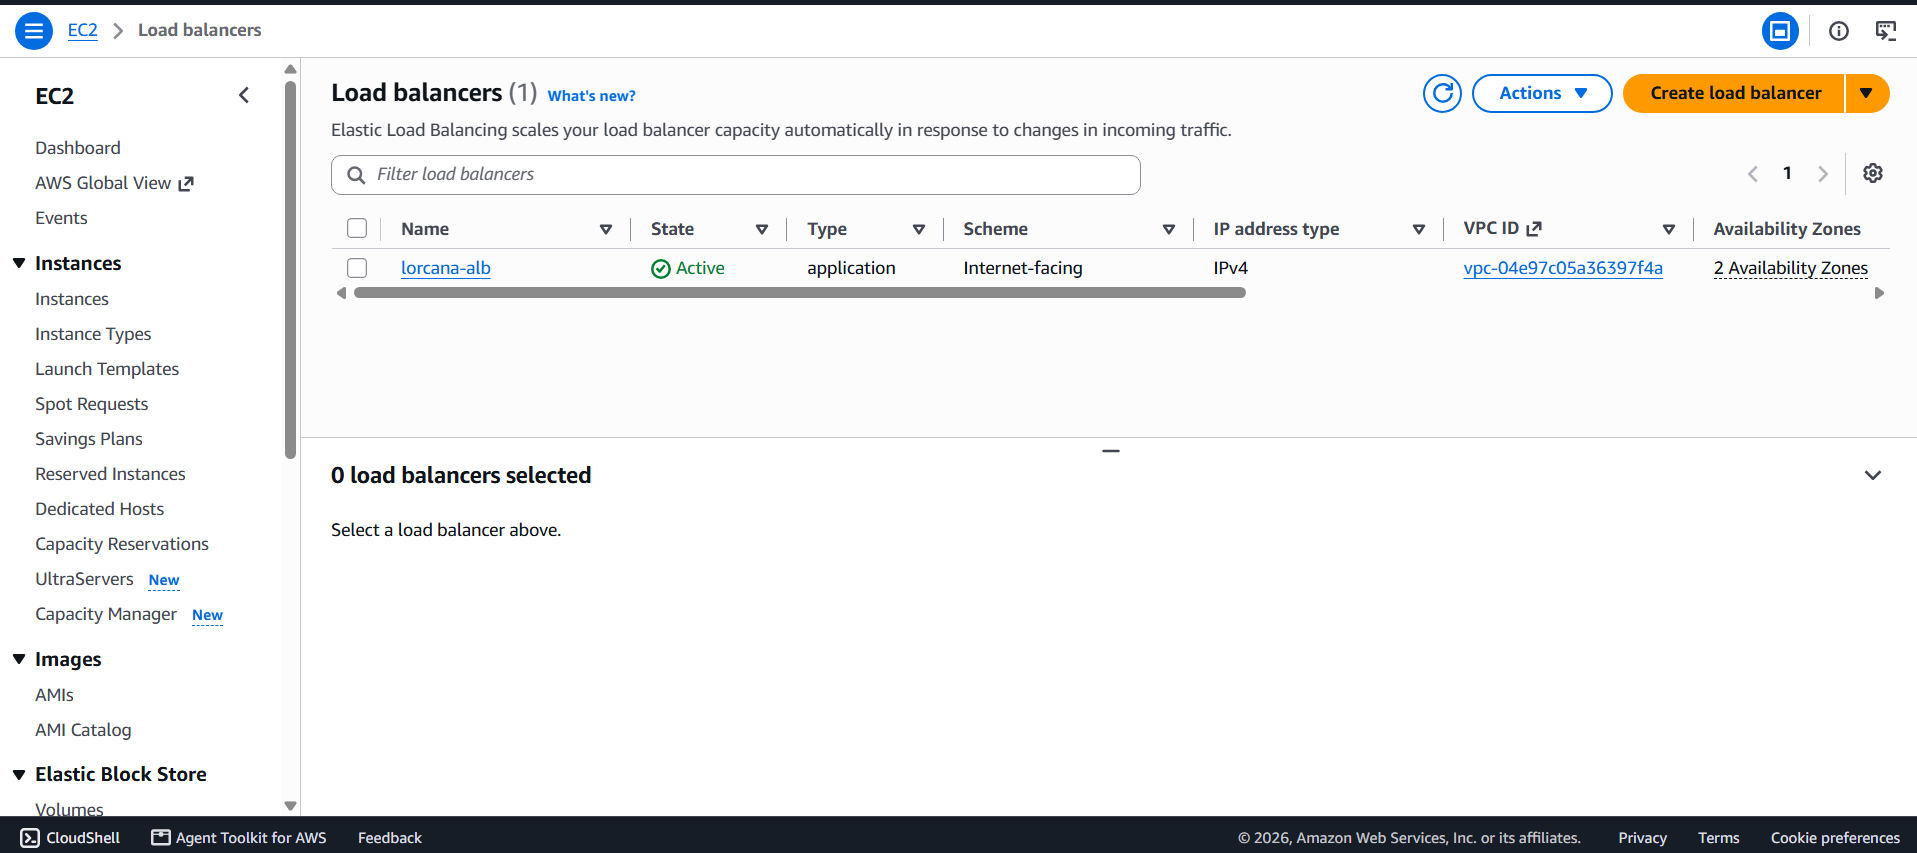
\includegraphics[width=\textwidth]{images/useindoc/aws_2026-10-12_alb_active.png}
    \caption{\texttt{lorcana-alb} สถานะ Active, Internet-facing, 2 Availability Zone}
\end{subfigure}
\hfill
\begin{subfigure}[b]{0.48\textwidth}
    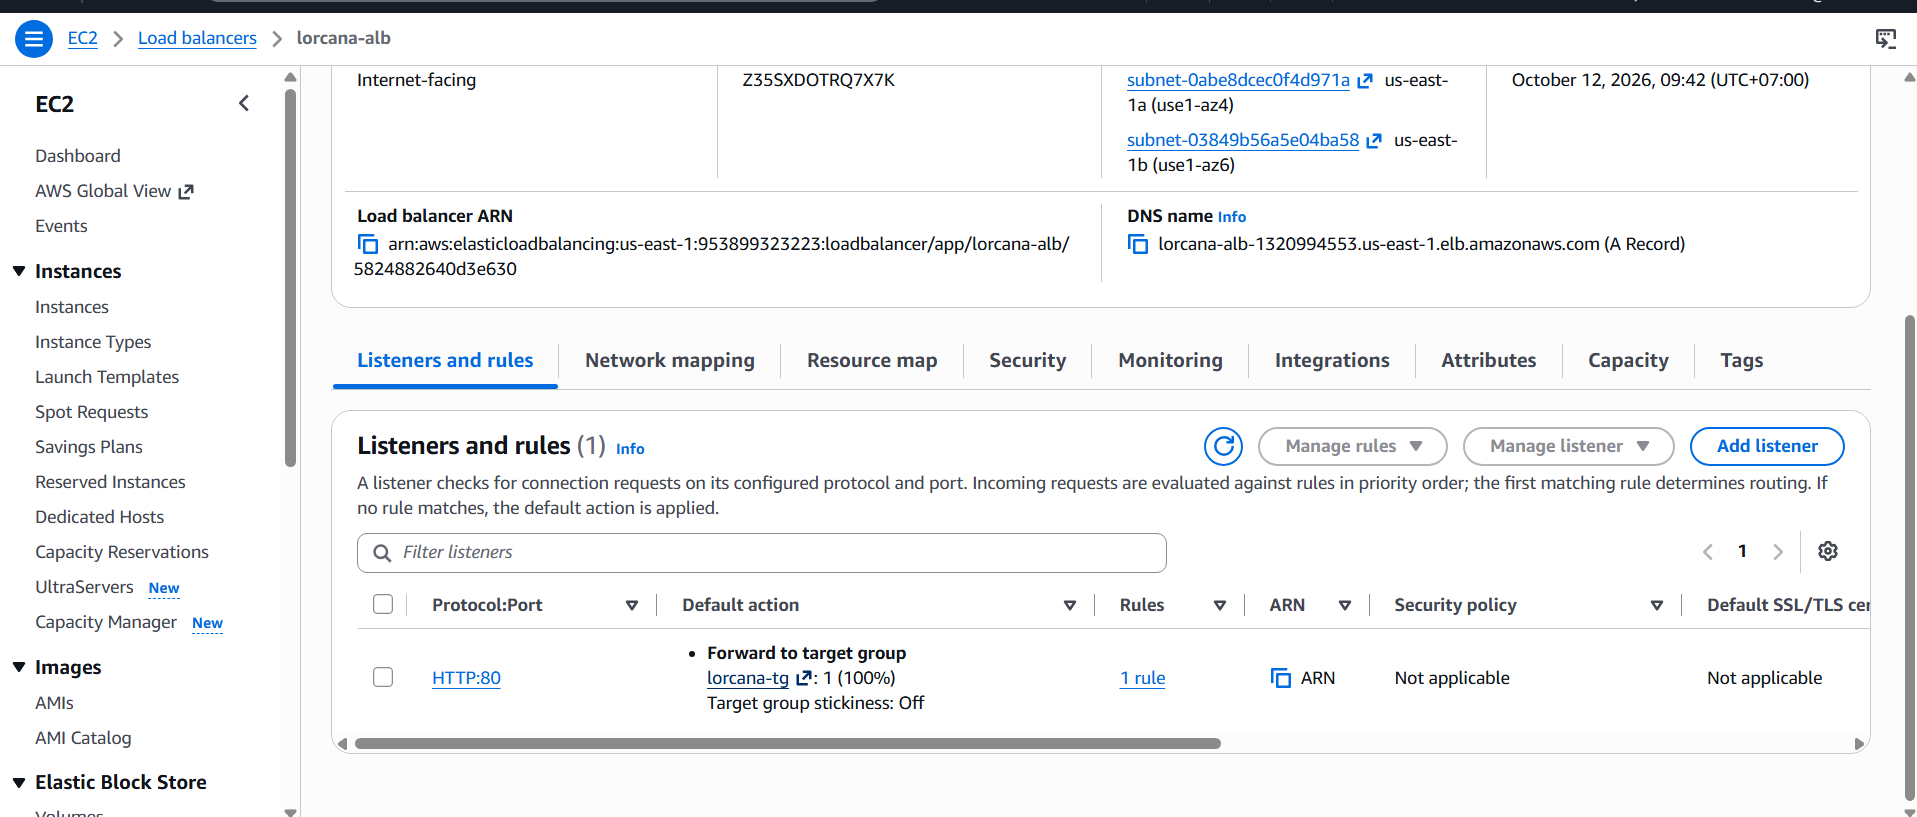
\includegraphics[width=\textwidth]{images/useindoc/aws_2026-10-12_alb_listener.png}
    \caption{Listener HTTP:80 ส่งต่อไปยัง target group \texttt{lorcana-tg}}
\end{subfigure}
\caption{Application Load Balancer ของระบบ}
\label{fig:aws_alb}
\end{figure}

\begin{figure}[H]
\centering
\begin{subfigure}[b]{0.48\textwidth}
    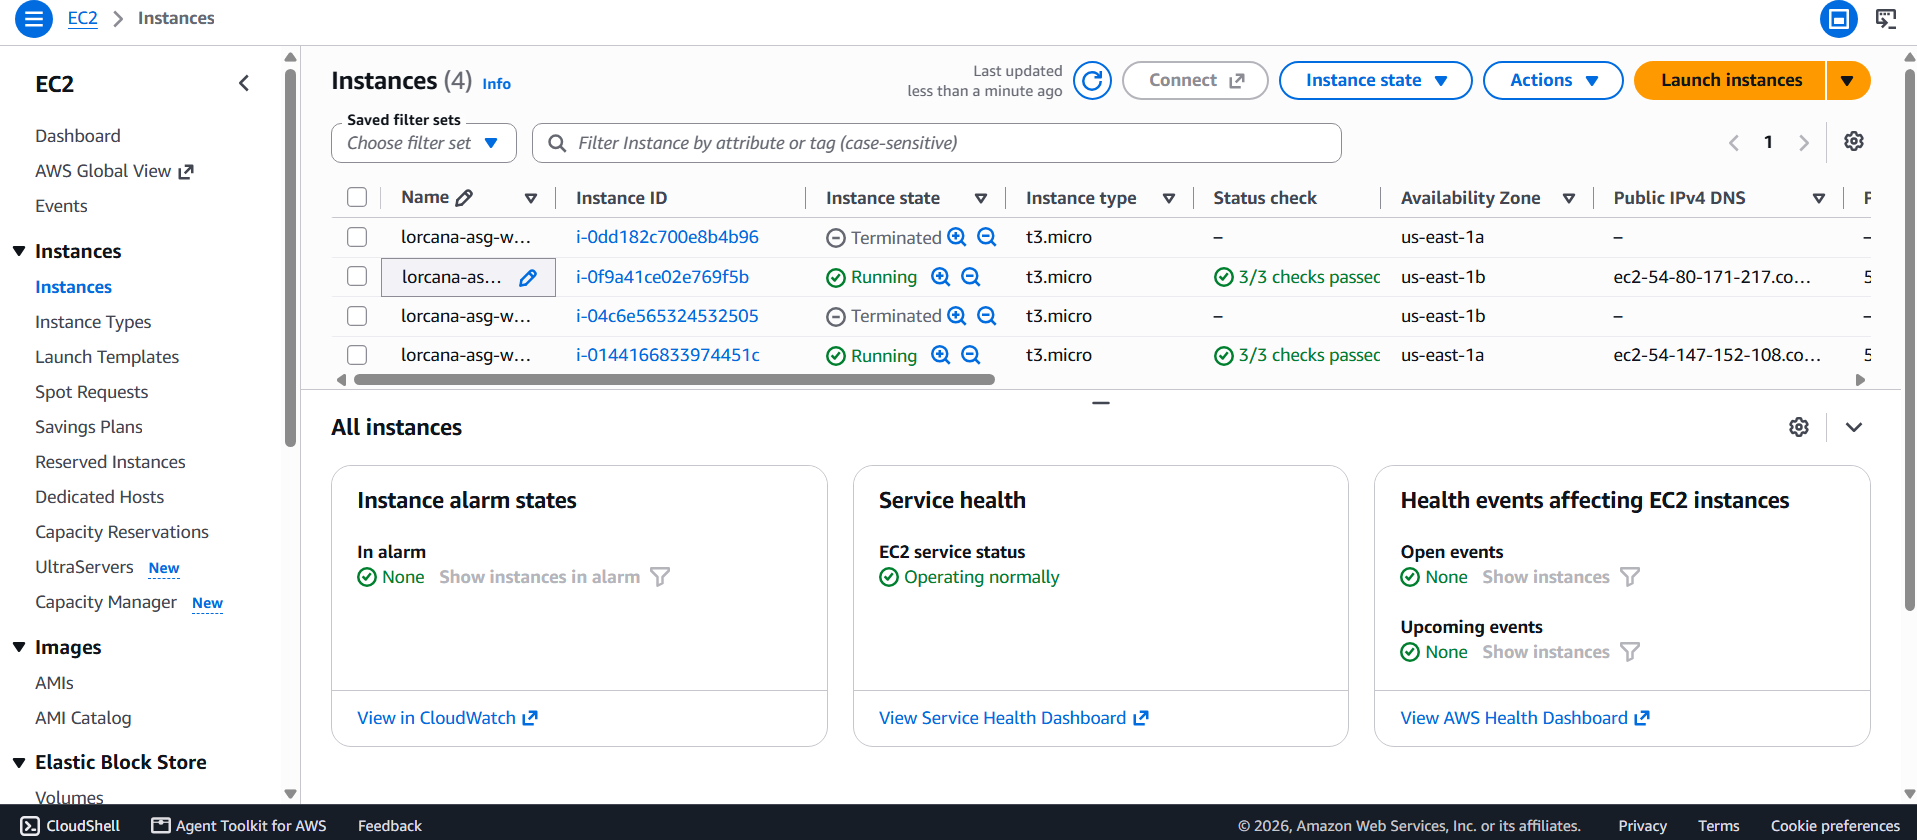
\includegraphics[width=\textwidth]{images/useindoc/aws_2026-10-12_ec2_instances.png}
    \caption{EC2 ที่กำลังทำงาน 2 เครื่อง ใน \texttt{us-east-1a} และ \texttt{us-east-1b} ผ่าน status check 3/3 ส่วนอีก 2 เครื่องเป็นเครื่องเก่าที่ถูกแทนที่ (Terminated)}
\end{subfigure}
\hfill
\begin{subfigure}[b]{0.48\textwidth}
    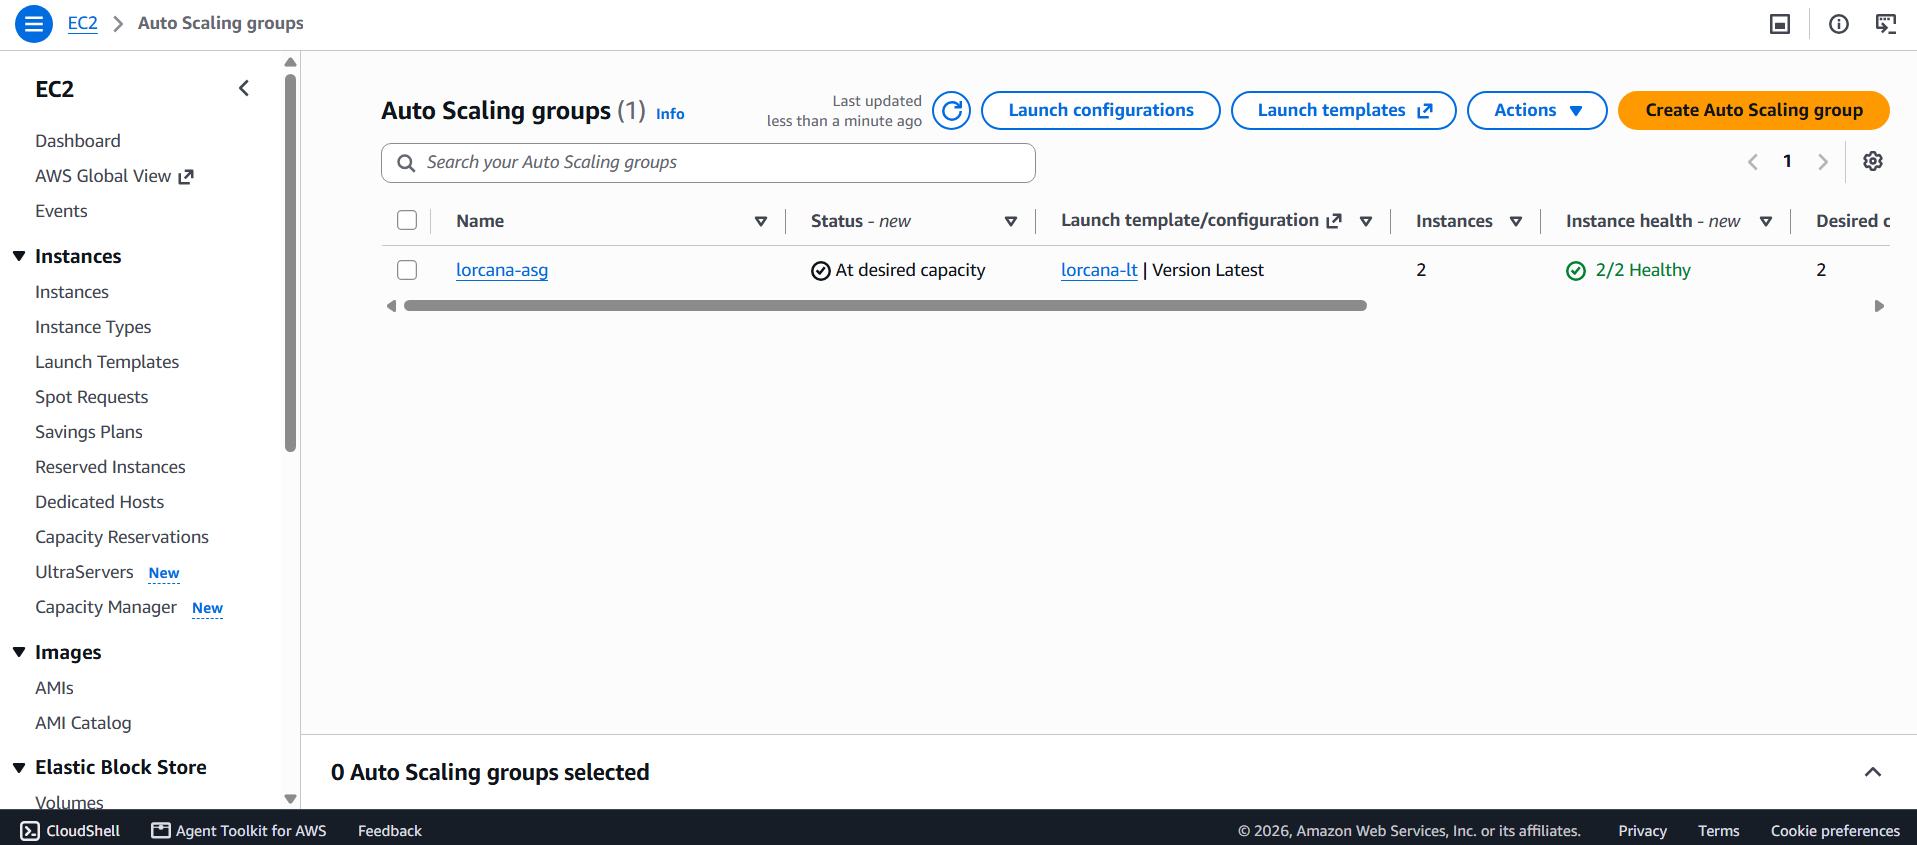
\includegraphics[width=\textwidth]{images/useindoc/aws_2026-10-12_asg_overview.png}
    \caption{Auto Scaling group \texttt{lorcana-asg} At desired capacity, 2 เครื่อง สถานะ 2/2 Healthy}
\end{subfigure}
\caption{เครื่อง EC2 และ Auto Scaling group}
\label{fig:aws_ec2_asg}
\end{figure}

\begin{figure}[H]
\centering
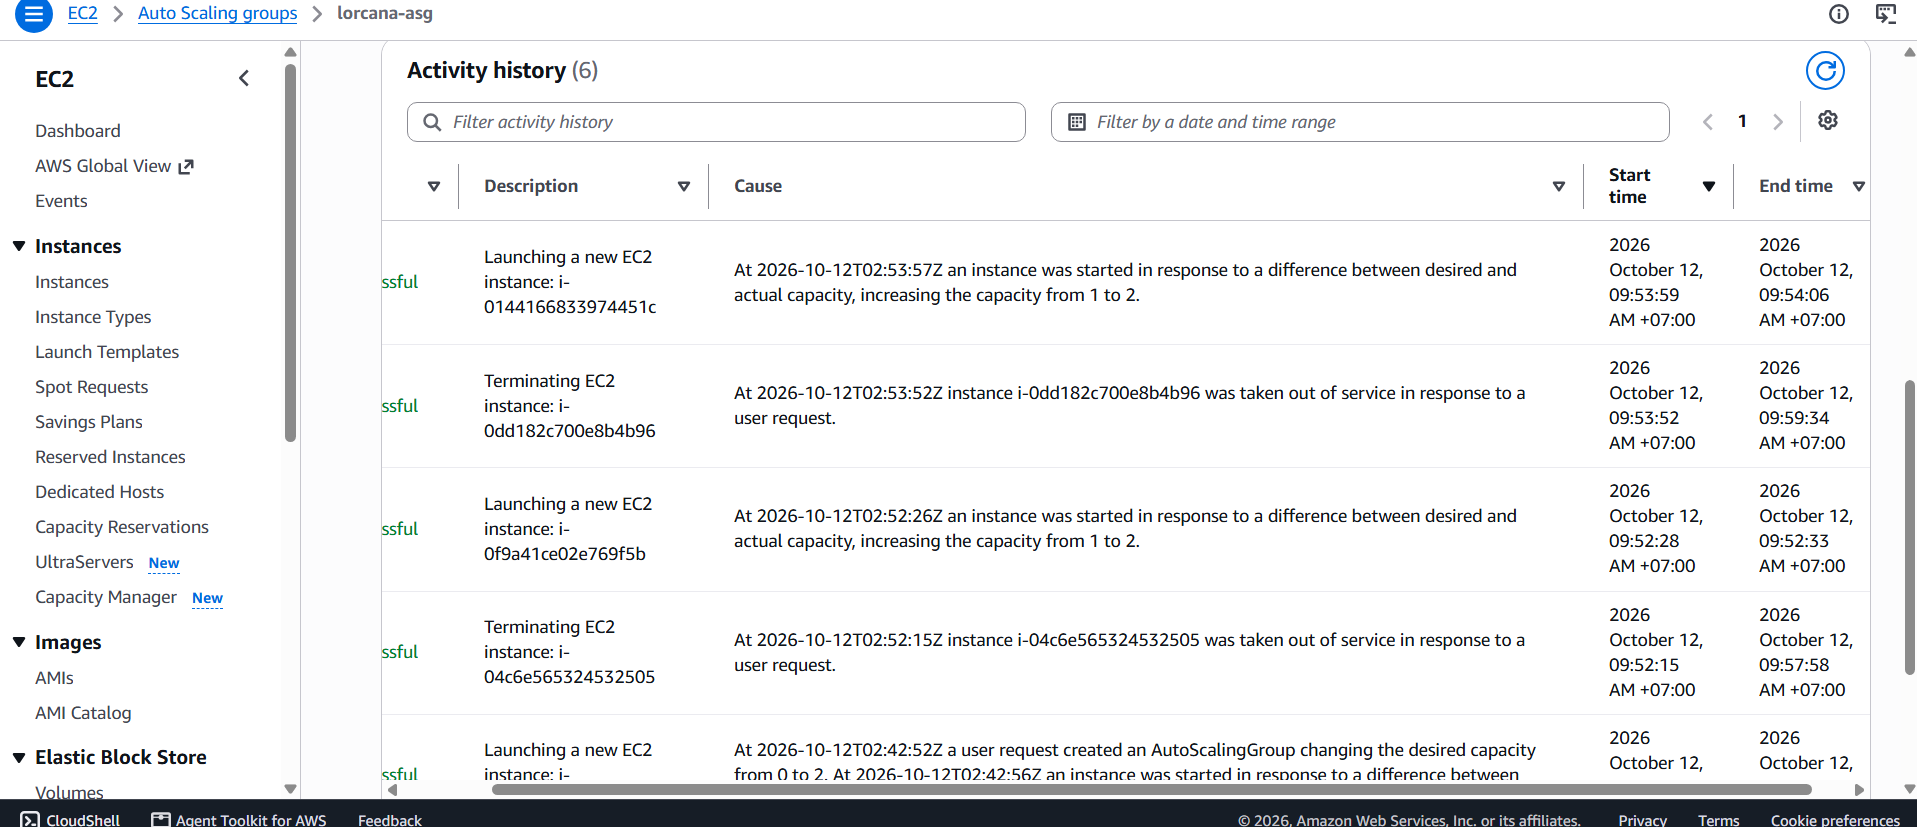
\includegraphics[width=\textwidth]{images/useindoc/aws_2026-10-12_asg_activity.png}
\caption{Activity history ของ \texttt{lorcana-asg}: การเปลี่ยนเครื่องทีละเครื่อง (terminate เครื่องเก่า แล้ว launch เครื่องใหม่ทดแทน) ระหว่าง \texttt{lab.ps1 publish} และการเพิ่มจำนวนเครื่องจาก 0 เป็น 2 เมื่อสร้าง stack}
\label{fig:aws_asg_activity}
\end{figure}

\begin{figure}[H]
\centering
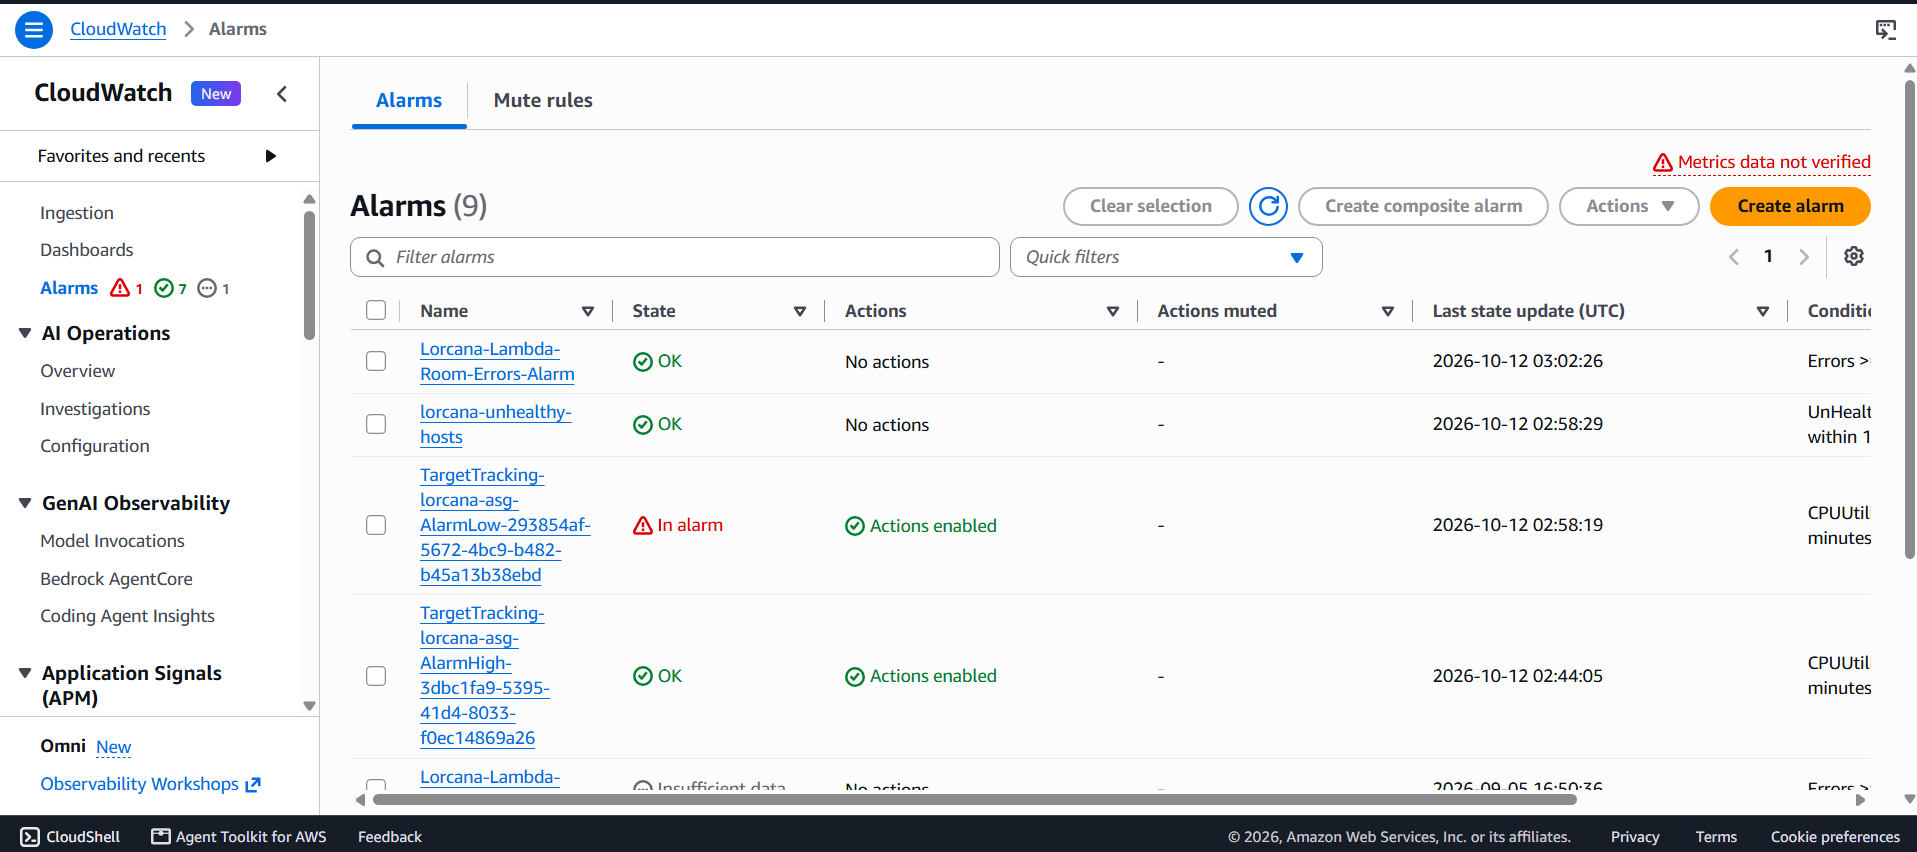
\includegraphics[width=\textwidth]{images/useindoc/aws_2026-10-12_cloudwatch_alarms.png}
\caption{CloudWatch Alarms: \texttt{lorcana-unhealthy-hosts} และ alarm ของ target tracking \texttt{AlarmHigh} อยู่สถานะ OK ส่วน \texttt{AlarmLow} อยู่สถานะ In alarm ตามปกติเมื่อโหลดต่ำ (CPU ต่ำกว่าเป้า) ระบบไม่ลดจำนวนเครื่องเพราะ MinSize เท่ากับ 2 ภาพนี้ไม่ใช่หลักฐานการเพิ่มเครื่อง}
\label{fig:aws_cloudwatch}
\end{figure}

\begin{figure}[H]
\centering
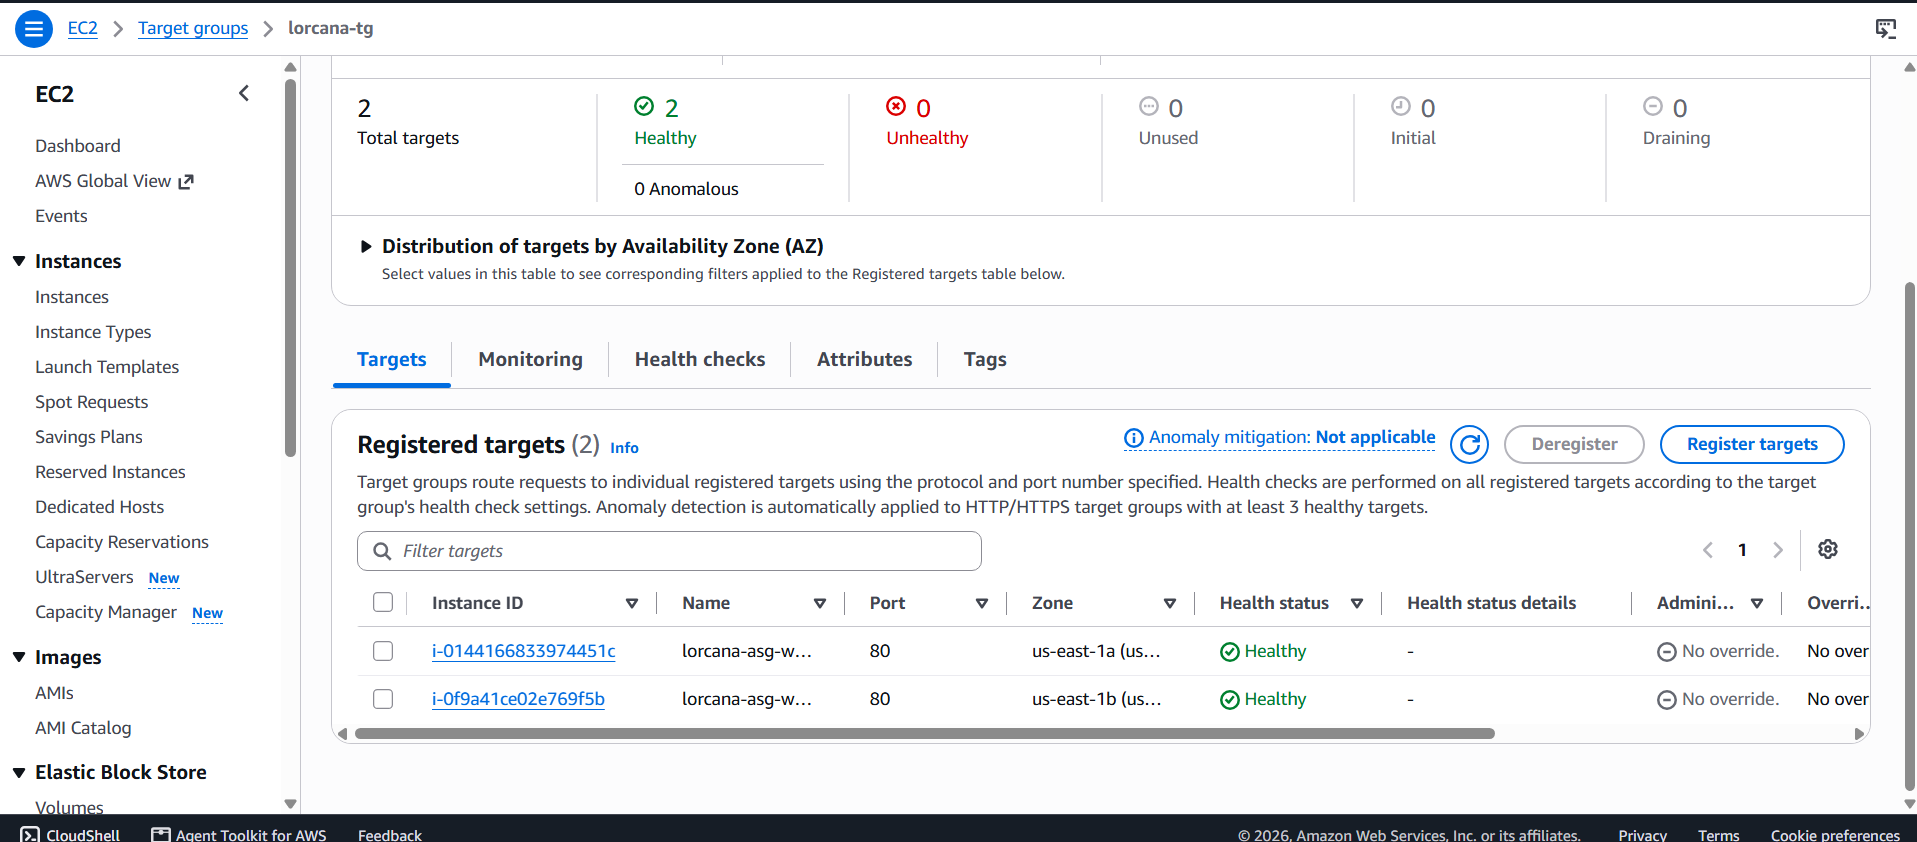
\includegraphics[width=\textwidth]{images/useindoc/aws_2026-10-12_target_group.png}
\caption{Target group \texttt{lorcana-tg} แท็บ Targets: 2 targets สถานะ Healthy 2 และ Unhealthy 0 เครื่องหนึ่งอยู่ใน \texttt{us-east-1a} และอีกเครื่องอยู่ใน \texttt{us-east-1b} พอร์ต 80}
\label{fig:aws_target_group}
\end{figure}

ภาพชุดนี้แสดงสถานะของ stack ขณะไม่มีโหลด จึงไม่มีภาพ alarm สั่งเพิ่มเครื่องจาก 2 เป็น 4 ผลการทดลองเรื่องการปรับจำนวนเครื่องตามโหลดอยู่ในไฟล์ข้อมูลของการทดลองเดิมใน \texttt{docs/01\_Reports/stage3\_evidence/} ซึ่งรันบน stack รุ่นก่อนหน้า

% =============================================================
\chapter{ข้อจำกัดและค่าใช้จ่าย}
\label{ch:limits}
% =============================================================

\section{ข้อจำกัดของระบบ}

\begin{enumerate}
    \item \textbf{ไม่มี HTTPS:} Learner Lab ไม่มีโดเมน จึงขอ certificate จาก ACM ให้ ALB ไม่ได้ ข้อมูลเข้าสู่ระบบส่งเป็น HTTP
    \item \textbf{WebSocket ไม่ตรวจ token:} Lambda \texttt{lorcana-room} เชื่อชื่อผู้ใช้ที่ client ส่งมา
    \item \textbf{Rate limiter อยู่ใน memory ของแต่ละ process (OWASP A07):} เมื่อมีหลาย worker และหลายเครื่อง ผู้โจมตีลองรหัสได้ 5 ครั้งคูณจำนวน worker คูณจำนวนเครื่อง แก้ได้ด้วย DynamoDB และ TTL แต่เพิ่มค่าใช้จ่ายต่อคำขอ
    \item \textbf{Secret ของ Lambda เป็น environment variable แบบ plaintext:} (EC2 อ่านจาก SSM SecureString)
    \item \textbf{เวลากู้คืน 2.8 ถึง 3.9 นาที:} ขึ้นกับเวลาบูตเครื่องใหม่
    \item \textbf{Alarm มาช้ากว่าเหตุการณ์ 2 ถึง 3 นาที:} metric ของ CloudWatch มาถึงช้า
    \item \textbf{ผลการแข่งขันรายงานจาก client:} ตัวขับเคลื่อนกฎทำงานในเบราว์เซอร์ ยังไม่มี authoritative game server ตรวจสถานะเกม
    \item \textbf{ElastiCache เป็น Node เดี่ยว:} เป็น single point of failure ของชั้นแคช (ระบบ fallback ไป DynamoDB)
    \item \textbf{CloudFront และ ElastiCache Serverless ใช้ไม่ได้:} นโยบาย IAM ของ Learner Lab ปฏิเสธ
    \item \textbf{Ability ที่ระบบจัดการอัตโนมัติเต็มรูปแบบมี 16.16\%:} ที่เหลือแสดงป้ายให้ผู้เล่นจัดการเอง
    \item \textbf{Session ของ Learner Lab ประมาณ 4 ชั่วโมง:} เครื่องถูกหยุดเมื่อหมด session
    \item \textbf{ค่าใช้จ่ายเมื่อเปิดต่อเนื่อง 24 ชั่วโมง:} ดูหัวข้อ \ref{sec:cost}
\end{enumerate}

\section{ประมาณการค่าใช้จ่าย}
\label{sec:cost}

ราคาต่อหน่วยเป็นราคา on-demand ของ us-east-1 \todo{ตรวจราคาทุกแถวกับหน้า AWS Pricing แล้วใส่วันที่เข้าถึงจริง รายงาน Phase 3 ระบุ "ตรวจสอบ 29 กันยายน 2569" แต่ Pricing API ถูกบล็อกใน Learner Lab จึงยังไม่มีการตรวจ}

\begin{table}[H]
\centering
\caption{ประมาณการค่าใช้จ่ายรายชั่วโมงเมื่อเปิด stack เต็มรูปแบบ}
\label{tab:cost_hourly}
\begin{tabularx}{\textwidth}{lXrr}
\toprule
\textbf{บริการ} & \textbf{ราคาต่อหน่วย} & \textbf{จำนวน} & \textbf{ต่อชม. (USD)} \\
\midrule
EC2 t3.micro & \$0.0104/ชม. & 2 & 0.0208 \\
EBS gp3 root 8 GiB & \$0.08/GB-เดือน & 2 $\times$ 8 GiB & 0.0018 \\
Public IPv4 & \$0.005/ชม. & 4 (EC2 2 และ ALB 2 AZ) & 0.0200 \\
ALB & \$0.0225/ชม. บวก LCU & 1 (1 LCU) & 0.0305 \\
ElastiCache t3.micro & \$0.0170/ชม. & 1 node & 0.0170 \\
Detailed monitoring & \$2.10/เครื่อง-เดือน & 2 & 0.0058 \\
CloudWatch alarm & \$0.10/alarm-เดือน & 3 & 0.0004 \\
SNS, SQS, Lambda, DynamoDB & ระดับทดสอบ & -- & $\approx$ 0.0000 \\
\midrule
\textbf{รวม} & & & \textbf{$\approx$ 0.096} \\
\bottomrule
\end{tabularx}
\end{table}

\begin{table}[H]
\centering
\caption{ค่าใช้จ่ายจริงจาก AWS Billing (1--27 กันยายน 2569)}
\label{tab:billing}
\begin{tabularx}{\textwidth}{lrr}
\toprule
\textbf{บริการ} & \textbf{ก.ย. 2569 (USD)} & \textbf{สัดส่วน} \\
\midrule
Elastic Load Balancing & 7.13 & 69\% \\
Amazon VPC (public IPv4) & 1.96 & 19\% \\
CloudWatch & 0.45 & 4\% \\
EC2 Compute & 0.44 & 4\% \\
EC2 Other (EBS) & 0.31 & 3\% \\
\midrule
\textbf{รวมตั้งแต่ต้นเดือน} & \textbf{10.29} & \\
\bottomrule
\end{tabularx}
\end{table}

ALB คิดเงินรายชั่วโมงตลอดเวลาที่ยังไม่ลบ แม้ EC2 จะถูกลดเหลือ 0 (\texttt{lab\_stop.ps1}) แล้ว ค่า Compute จึงหยุดได้ แต่ค่า ALB, Public IPv4 ของ ALB และ ElastiCache ไม่หยุด หากหยุดทดสอบเกิน 1 วัน ควรสั่ง \texttt{lab.ps1 destroy} ข้อสังเกตนี้แทนข้อความ "Scale-to-Zero ทำให้ค่าใช้จ่ายเป็น \$0.00 ต่อชั่วโมง" ในรายงานระยะที่ 2 ซึ่งใช้ได้กับค่า EC2 เท่านั้น

\subsection{ยอดค่าใช้จ่ายทั้งเดือนกันยายน 2569}

หน้า Billing and Cost Management เมื่อวันที่ 5 ตุลาคม 2569 (รูปที่ \ref{fig:billing}) แสดงค่าใช้จ่ายรวมของเดือนกันยายนทั้งเดือน 13.49 ดอลลาร์ ซึ่งสูงกว่ายอด 10.29 ดอลลาร์ในตารางที่ \ref{tab:billing} ที่นับถึงวันที่ 27 กันยายน ส่วนต่าง 3.20 ดอลลาร์เป็นค่าใช้จ่ายของวันที่ 28 ถึง 30 กันยายน ค่า CloudWatch เดือนกันยายนในภาพคือ 0.69 ดอลลาร์ และกลุ่ม Others 12.79 ดอลลาร์ ภาพนี้ไม่แยกกลุ่ม Others เป็นรายบริการ ตารางที่ \ref{tab:billing_full} จึงใช้ข้อมูลจาก AWS Cost Explorer API (\texttt{aws ce get-cost-and-usage}) ที่ดึงเมื่อวันที่ 5 ตุลาคม 2569 โดยกรองเฉพาะรายการประเภท Usage

\begin{figure}[H]
\centering
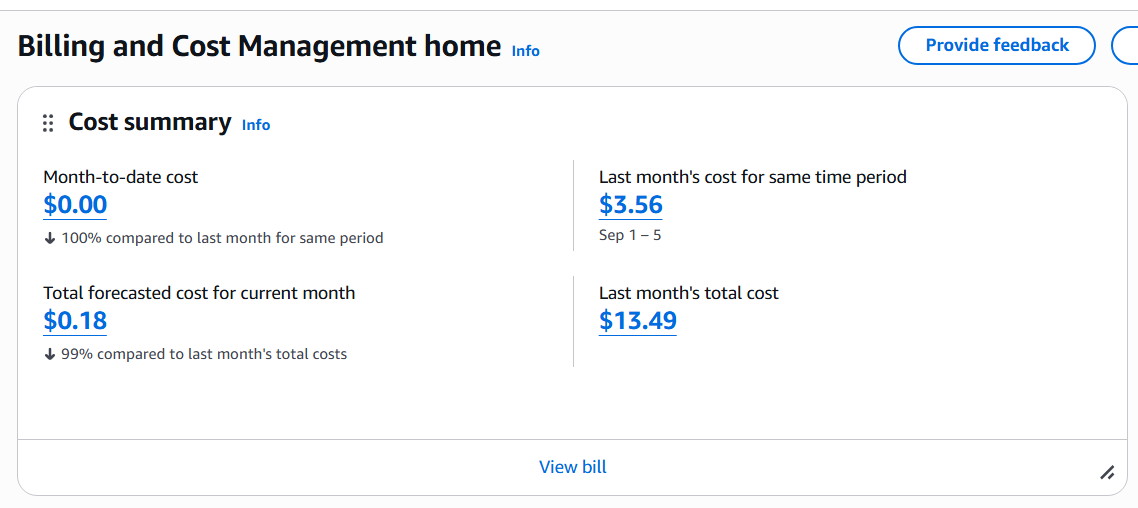
\includegraphics[width=0.78\textwidth]{images/useindoc/billing_cost_summary_2026-10-05.png}\\[0.3cm]
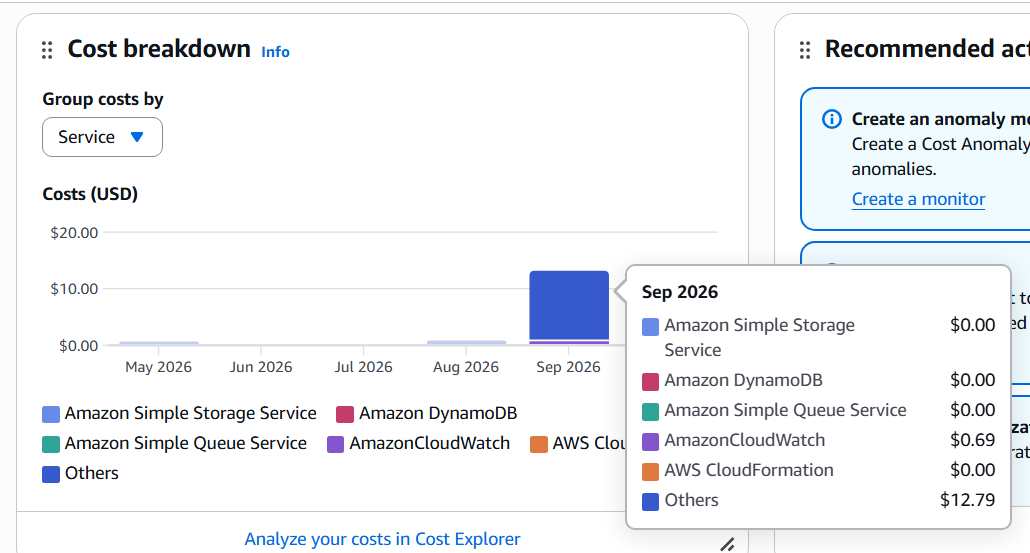
\includegraphics[width=0.78\textwidth]{images/useindoc/billing_cost_breakdown_2026-10-05.png}
\caption{หน้า Billing and Cost Management (5 ตุลาคม 2569): ยอดเดือนกันยายน 13.49 ดอลลาร์ และสัดส่วนตามบริการ}
\label{fig:billing}
\end{figure}

ค่าใช้จ่ายเดือนตุลาคมที่แสดงเป็น 0.00 ดอลลาร์ในภาพเป็นเพราะข้อมูล Billing ล่าช้ากว่าการใช้งานจริง stack ที่ deploy เมื่อวันที่ 5 ตุลาคม ยังไม่ปรากฏในยอดนี้

\begin{table}[H]
\centering
\caption{ค่าใช้จ่ายการใช้งาน (Usage) เดือนกันยายน 2569 ทั้งเดือน แยกตามบริการ (Cost Explorer API)}
\label{tab:billing_full}
\begin{tabularx}{\textwidth}{lrr}
\toprule
\textbf{บริการ} & \textbf{USD} & \textbf{สัดส่วน} \\
\midrule
Elastic Load Balancing & 7.72 & 57.3\% \\
Amazon VPC (public IPv4) & 2.36 & 17.5\% \\
EC2-Other (EBS, NAT Gateway ฯลฯ) & 1.18 & 8.8\% \\
EC2 Compute & 0.94 & 6.9\% \\
CloudWatch & 0.69 & 5.1\% \\
Amazon RDS & 0.50 & 3.7\% \\
ElastiCache & 0.07 & 0.5\% \\
AWS Cost Explorer & 0.02 & 0.1\% \\
S3, DynamoDB, API Gateway, KMS, EventBridge & 0.01 & 0.1\% \\
\midrule
\textbf{รวมค่าใช้งาน} & \textbf{13.49} & \\
เครดิตของบัญชี (Credit) & $-$13.49 & \\
\textbf{ยอดสุทธิ} & \textbf{0.00} & \\
\bottomrule
\end{tabularx}
\end{table}

ข้อสังเกตจากตารางที่ \ref{tab:billing_full}:
\begin{itemize}
    \item ค่า Elastic Load Balancing เกือบทั้งหมด (7.72 จาก 7.72 ดอลลาร์) เป็น \texttt{LoadBalancerUsage} หรือค่าชั่วโมงที่ ALB เปิดอยู่ ส่วนค่า LCU ตามปริมาณทราฟฟิกมีเพียง 0.006 ดอลลาร์
    \item ค่าใช้จ่ายรวมของเดือนสิงหาคมคือ 0.82 ดอลลาร์ และของวันที่ 1--5 ตุลาคมคือ 0.0002 ดอลลาร์ (ข้อมูลล่าช้า) รวมตั้งแต่ 1 สิงหาคมถึง 5 ตุลาคมประมาณ 14.31 ดอลลาร์ก่อนหักเครดิต
    \item ตัวเลขสุทธิเป็น 0 เพราะรายการ Credit หักค่าใช้งานทั้งหมด หน้า Billing Console แสดงยอดก่อนหักเครดิต (13.49) ส่วนรายงานจาก Cost Explorer ที่ไม่กรองประเภทรายการ และผลของ Amazon Q ที่ตอบเกือบ 0 ดอลลาร์ แสดงยอดสุทธิหลังหักเครดิต
    \item \textbf{ค่า EC2-Other มี NAT Gateway ประมาณ 13 ชั่วโมง (0.585 ดอลลาร์ ที่อัตรา 0.045 ดอลลาร์ต่อชั่วโมง) และข้อมูลผ่าน NAT อีก 0.19 ดอลลาร์ และมีค่า Amazon RDS 0.50 ดอลลาร์} สคริปต์ของโครงงานไม่สร้างทั้งสองอย่าง และขณะตรวจเมื่อวันที่ 5 ตุลาคม 2569 ไม่มี NAT Gateway หรือ RDS instance อยู่ในบัญชี AWS CloudTrail บันทึกว่าทั้งสองอย่างถูกสร้างเมื่อวันที่ 28 กันยายน 2569 เวลา 01:37 น. (NAT Gateway) และ 01:38 น. (RDS) โดย IAM user เดียวกับที่ใช้ deploy โครงงาน ห่างกัน 1 นาที ไม่ได้มาจากสคริปต์ของโครงงาน \todo{ระบุว่า NAT Gateway และ RDS ที่สร้างเมื่อ 28 ก.ย. 01:37 น. เป็นของงานอะไร (เช่น lab อื่นหรือการลองใน Console) เพื่อเขียนว่าเป็นค่าใช้จ่ายนอกโครงงาน}
\end{itemize}

% =============================================================
\chapter{สรุปและข้อเสนอแนะ}
\label{ch:summary}
% =============================================================

\section{สรุปผลการดำเนินงาน}

ระบบ Disney Lorcana PlayLab Cloud ทำงานได้ครบตามขอบเขตในบทที่ 1 และมีหลักฐานการวัดผลบน AWS ดังนี้

\begin{enumerate}
    \item \textbf{ระยะที่ 2:} หน้าเว็บ ระบบสมาชิก จัดการเด็ค ห้องเล่นเรียลไทม์ และโครงสร้าง Multi-AZ (VPC, ALB, ASG)
    \item \textbf{Content Caching:} ลดขนาดการรับส่งไฟล์ข้อมูลการ์ด 81.43\% และเวลาโหลดซ้ำจาก 602 เหลือ 86 มิลลิวินาที
    \item \textbf{Dead Letter Queue:} ข้อความที่ประมวลผลล้มเหลวเข้า DLQ ภายใน 102 วินาที โดยไม่ค้างในคิวหลัก
    \item \textbf{SNS Fan-out:} ผลการแข่งขันปรากฏในประวัติและสถิติของทั้งสองผู้เล่นภายใน 5 วินาที พร้อมป้องกันการนับซ้ำ
    \item \textbf{ElastiCache Cache-Aside:} เวลาประมวลผลฝั่ง server ของตารางผู้นำลดจาก 41 เหลือ 1 มิลลิวินาที (ค่ามัธยฐาน) และมี fallback เมื่อแคชใช้ไม่ได้
    \item \textbf{Failover และ Auto Scaling:} แทนเครื่องที่ล่มได้ใน 2.8 ถึง 3.9 นาที และขยายจาก 2 เป็น 4 เครื่องเมื่อใช้ Node.js cluster
    \item \textbf{ตัวขับเคลื่อนกฎเกม:} รองรับ 16 action types, 14 คีย์เวิร์ด, Ability 10 ประเภท, Shift, Location, Song และ Item ผ่านชุดทดสอบอัตโนมัติ 128 รายการ
\end{enumerate}

ค่าใช้งานเดือนกันยายนทั้งเดือน 13.49 ดอลลาร์ก่อนหักเครดิต อยู่ภายในงบ 50 ดอลลาร์

\section{บทเรียนที่ได้รับ}

\begin{enumerate}
    \item \textbf{ค่าใช้จ่ายขึ้นกับทรัพยากรที่คิดรายชั่วโมง:} ALB คิดเป็น 57\% ของค่าใช้งานเดือนกันยายน การลด EC2 เป็น 0 ไม่หยุดค่า ALB
    \item \textbf{ออกแบบเผื่อหลายเครื่อง:} WebSocket ที่เก็บ state ใน memory ใช้ไม่ได้เมื่อมี 2 เครื่อง ต้องย้ายสถานะไป DynamoDB
    \item \textbf{เป้าหมาย scaling ต้องใช้ CPU ได้ถึงเป้า:} Node.js แบบ process เดียวใช้ CPU ได้ราวครึ่งเดียวของ t3.micro เป้า 60\% จึงไม่ถูกกระตุ้นจนกว่าจะใช้ cluster
    \item \textbf{สคริปต์ต้องตรวจผลหลังรันทุกครั้ง:} บั๊กชื่อ key ตาราง (การทดลองที่ 5) ผ่านการสร้างโดยไม่มี error แต่ทำให้ Lambda เขียนตารางไม่ได้ จึงควรมีขั้นตรวจ schema หลังสร้าง
    \item \textbf{เอกสารต้องตรวจกับระบบจริง:} รายงานระยะที่ 2 ระบุขนาด ASG และการรัน Docker ที่ไม่ตรงกับสคริปต์ที่ใช้ deploy จริง รายงานฉบับนี้แก้ให้ตรงและอ้างไฟล์หลักฐานทุกค่า
\end{enumerate}

\section{ข้อเสนอแนะ}

\begin{enumerate}
    \item ย้าย rate limiter จาก memory ไปใช้ DynamoDB พร้อม TTL เพื่อแก้ปัญหา OWASP A07
    \item เพิ่มเซิร์ฟเวอร์ตรวจสถานะเกม (authoritative game state) เพื่อป้องกันผลการแข่งขันที่ถูกแก้จาก client
    \item หากมีโดเมน ให้เพิ่ม HTTPS ผ่าน ACM และ ALB listener พอร์ต 443
    \item เพิ่มสัดส่วน Ability ที่รองรับเต็มรูปแบบจาก 16.16\% โดยเริ่มจากกลุ่ม trigger ที่พบมาก (activated 412 ข้อ, on\_play 596 ข้อ)
    \item หากใช้นอก Learner Lab ให้พิจารณา CloudFront และ ElastiCache Serverless
    \item เพิ่มการตรวจ schema ตารางหลังสร้างใน \texttt{ensure\_pipeline.ps1}
\end{enumerate}

% -------------------------------------------------------------
% REFERENCES
% -------------------------------------------------------------
\chapter*{บรรณานุกรม (References)}
\addcontentsline{toc}{chapter}{บรรณานุกรม (References)}

\noindent [1] Ravensburger \& Disney. (n.d.). \textit{Disney Lorcana Comprehensive Rules v2.2.0}. [Online]. Available: \url{https://www.disneylorcana.com/resources} (ไฟล์ที่ใช้อยู่ที่ \nolinkurl{docs/Rule/Comprehensive-Rules_2.2.0-EN.pdf})\\[0.3cm]
\noindent [2] Amazon Web Services. (2026). \textit{Amazon SNS and SQS Fanout Pattern}. [Online]. Available: \url{https://docs.aws.amazon.com/sns/latest/dg/sns-sqs-as-subscriber.html}\\[0.3cm]
\noindent [3] Amazon Web Services. (2026). \textit{Amazon SQS Dead-Letter Queues}. Amazon SQS Developer Guide. [Online]. Available: \url{https://docs.aws.amazon.com/AWSSimpleQueueService/latest/SQSDeveloperGuide/sqs-dead-letter-queues.html}\\[0.3cm]
\noindent [4] Amazon Web Services. (2026). \textit{Amazon ElastiCache for Valkey}. [Online]. Available: \url{https://docs.aws.amazon.com/AmazonElastiCache/latest/dg/WhatIs.html}\\[0.3cm]
\noindent [5] Vite. (2026). \textit{Building for Production: Asset Hashing}. [Online]. Available: \url{https://vite.dev/guide/build}\\[0.3cm]
\noindent [6] OpenJS Foundation. (2026). \textit{Cluster Module}. Node.js Documentation. [Online]. Available: \url{https://nodejs.org/api/cluster.html}\\[0.3cm]
\noindent [7] Amazon Web Services. (2026). \textit{Target Tracking Scaling Policies for Amazon EC2 Auto Scaling}. [Online]. Available: \url{https://docs.aws.amazon.com/autoscaling/ec2/userguide/as-scaling-target-tracking.html}\\[0.3cm]
\noindent [8] Amazon Web Services. (2026). \textit{Health Checks for Application Load Balancer Target Groups}. [Online]. Available: \url{https://docs.aws.amazon.com/elasticloadbalancing/latest/application/target-group-health-checks.html}\\[0.3cm]
\noindent [9] Amazon Web Services. (2026). \textit{AWS Systems Manager Parameter Store}. [Online]. Available: \url{https://docs.aws.amazon.com/systems-manager/latest/userguide/systems-manager-parameter-store.html}\\[0.3cm]
\noindent [10] OWASP Foundation. (2021). \textit{OWASP Top 10: 2021}. [Online]. Available: \url{https://owasp.org/www-project-top-ten/}\\[0.3cm]
\noindent [11] Amazon Web Services. (2026). \textit{Amazon VPC Pricing (Public IPv4 Charges)}. [Online]. Available: \url{https://aws.amazon.com/vpc/pricing/}\\[0.3cm]
\noindent [12] Amazon Web Services. (2026). \textit{AWS Well-Architected Framework}. [Online]. Available: \url{https://aws.amazon.com/architecture/well-architected/}

% -------------------------------------------------------------
% APPENDIX
% -------------------------------------------------------------
\chapter*{ภาคผนวก (Appendix)}
\addcontentsline{toc}{chapter}{ภาคผนวก (Appendix)}

\section*{ภาคผนวก ก: ส่วนสร้าง Launch Template และ Auto Scaling Group ใน \texttt{scripts/deploy\_ec2\_vpc\_asg.ps1}}

\begin{lstlisting}[caption={ส่วนสร้าง ASG และ scaling policy (ตัดตอนจากสคริปต์จริง)}]
# Create ASG (Min: 2, Max: 4, Desired: 2) - Multi-AZ
aws autoscaling create-auto-scaling-group `
    --auto-scaling-group-name "lorcana-asg" `
    --launch-template "LaunchTemplateName=lorcana-lt,Version=`$Latest" `
    --min-size 2 `
    --max-size 4 `
    --desired-capacity 2 `
    --target-group-arns $TargetGroupArn `
    --vpc-zone-identifier "$Subnet1Id,$Subnet2Id" `
    --health-check-type "ELB" `
    --health-check-grace-period 120 `
    --region $Region

# Target Tracking Scaling Policy (CPU > 60%)
$policyConfig = @{
    TargetValue = 60.0
    PredefinedMetricSpecification = @{
        PredefinedMetricType = "ASGAverageCPUUtilization"
    }
    DisableScaleIn = $false
} | ConvertTo-Json -Compress
\end{lstlisting}

\section*{ภาคผนวก ข: สคริปต์ที่ใช้ในโครงงาน}

\begin{table}[H]
\centering
\caption{สคริปต์ในโฟลเดอร์ \texttt{scripts/}}
\small
\begin{tabularx}{\textwidth}{lX}
\toprule
\textbf{สคริปต์} & \textbf{หน้าที่} \\
\midrule
\texttt{deploy\_ec2\_vpc\_asg.ps1} & สร้าง VPC, Subnet, Security Group, ALB, Launch Template, ASG, scaling policy และ alarm (หยุดหากมี VPC เดิมอยู่) \\
\texttt{ensure\_pipeline.ps1} & สร้างคิว SQS, DLQ, SNS topic, ตาราง DynamoDB และ Lambda ของ pipeline แบบ idempotent \\
\texttt{ensure\_cache.ps1} & สร้างทรัพยากร ElastiCache \\
\texttt{lab.ps1} & คำสั่ง \texttt{start}, \texttt{stop}, \texttt{status}, \texttt{publish}, \texttt{lambdas}, \texttt{destroy} \\
\texttt{test\_asg\_recovery.ps1} & จำลองเครื่องล่มและจับเวลากู้คืน (การทดลองที่ 3) \\
\texttt{test\_dlq.ps1} & ทดสอบ Dead Letter Queue (การทดลองที่ 7) \\
\texttt{stress\_test.ps1} & สร้างโหลดเพื่อทดสอบ Auto Scaling (การทดลองที่ 4) \\
\texttt{measure\_leaderboard.mjs} & วัด MISS/HIT ของตารางผู้นำ (การทดลองที่ 9) \\
\texttt{measure\_ability\_coverage.ts} & วัดการรองรับ Ability ของการ์ด 3,242 ใบ (การทดลองที่ 10) \\
\texttt{build\_final\_report.py} & สร้างรายงานฉบับนี้เป็น PDF และ DOCX จากไฟล์ \texttt{.tex} \\
\bottomrule
\end{tabularx}
\end{table}


\end{document}
